%************************************************
\chapter[Appendix 2: Chapter 2 - Supplementary materials]{Appendix 2: Chapter 2
- Supplementary materials}\label{ch:Appendix2.1}
%************************************************

\renewcommand{\thefigure}{A.2.\arabic{figure}}
\setcounter{figure}{0}

\renewcommand{\thetable}{A.2.\arabic{table}}
\setcounter{table}{0}

\section*{Supplementary tables}

\begin{table}[ht!]
\center
\caption[FS PCs models]{
Characteristics of the models used to select the PCs that better describe the
generation time or elasticity to the fecundity. This models are used to
define the fast-slow axes averaging and AIC weighting the PCs from the models
predicting the elasticity to the fecundity (FSe) or generation time (FSgt)
for each dataset and phylogeny. Columns describe the number of PCs included (n
PCs), the variance explained by the PCs (PCvarExp), number of traits included in
the PPCAs and the adjusted $R^{2}$ of the models predicting the elasticity to
the fecundity or the generation time. Best AIC models include only the PCs
with $\Delta AIC < 2$. The values with variability among PCs are reported as the
mean $\pm$ standard deviation. See the ESM for the complete data for all the
models.
}
\label{tab:tabApp2.1}
\begin{tabular}{@{}lllllll@{}}
\toprule
Axis & Phylogeny & Dataset & n PCs & PCvarExp & n traits & adjusted $R^{2}$\\
\midrule
\multirow{4}{*}{FSe} & \multirow{2}{*}{Ericson} & maxN & $7616$ & $0.34\pm0.08$ & $7.29\pm1.51$ & $0.36\pm0.11$\\
 &  & restricSet & $7616$ & $0.35\pm0.07$ & $7.29\pm1.51$ & $0.36\pm0.11$\\
 & \multirow{2}{*}{Hackett}& maxN & $7616$ & $0.35\pm0.07$ & $7.29\pm1.51$ & $0.36\pm0.11$\\
 &  & restricSet & $7616$ & $0.35\pm0.07$ & $7.29\pm1.51$ & $0.36\pm0.11$\\
\addlinespace
\multirow{4}{*}{FSe best AIC} & \multirow{2}{*}{Ericson} & maxN & $61$ &
$0.28\pm0.05$ & $6.02\pm1.09$ & $0.55\pm0.01$\\
 &  & restricSet & $59$ & $0.28\pm0.05$ & $6\pm1.11$ & $0.55\pm0.01$\\
 & \multirow{2}{*}{Hackett} & maxN & $55$ & $0.28\pm0.05$ & $5.98\pm1.13$ & $0.55\pm0.01$\\
 &  & restricSet & $103$ & $0.3\pm0.05$ & $5.91\pm1.2$ & $0.55\pm0.01$\\
\addlinespace
\multirow{4}{*}{FSgt} & \multirow{2}{*}{Ericson} & maxN & $7616$ & $0.34\pm0.08$ & $7.29\pm1.51$ & $0.39\pm0.06$\\
 &  & restricSet & $7616$ & $0.35\pm0.08$ & $7.29\pm1.51$ & $0.39\pm0.06$\\
 & \multirow{2}{*}{Hackett} & maxN & $7616$ & $0.35\pm0.08$ & $7.29\pm1.51$ & $0.39\pm0.05$\\
 &  & restricSet & $7616$ & $0.35\pm0.07$ & $7.29\pm1.51$ & $0.39\pm0.05$\\
\addlinespace
\multirow{4}{*}{FSgt best AIC} & \multirow{2}{*}{Ericson} & maxN & $515$ &
$0.33\pm0.07$ & $6.27\pm1.29$ & $0.48\pm0.01$\\
 &  & restricSet & $499$ & $0.33\pm0.06$ & $6.26\pm1.28$ & $0.48\pm0.01$\\
 & \multirow{2}{*}{Hackett} & maxN & $497$ & $0.33\pm0.07$ & $6.23\pm1.27$ & $0.48\pm0.01$\\
 &  & restricSet & $468$ & $0.34\pm0.06$ & $6.24\pm1.28$ & $0.48\pm0.01$\\
\bottomrule
\end{tabular}
\end{table}


\clearpage% Flush earlier floats (otherwise order might not be correct)
\begin{landscape}
\begin{table}
\center
\caption[LHT loadings of the FS axes]{
Mean $\pm$ standard deviation AIC weighted loadings of the traits for the
fast-slow axes based on models predicting generation time (FSgt) or elasticity
to the fecundity (FSe) for all trait combination PCs o using only the PCs
with AIC \textless{2} (best AIC).
}
\label{tab:tabApp2.2}
\begin{footnotesize}

\textbf{Phylogeny based on Ericson backbone}

\begin{tabular}{@{}l|rrrr|rrrr@{}}
\toprule
  & \multicolumn{4}{c|}{Restricted Set} & \multicolumn{4}{c}{Max N Set}\\
  & FSe & FSe best AIC & FSgt & FSgt best AIC & FSe & FSe best AIC & FSgt & FSgt best AIC\\
\midrule
CS & $-0.44 \pm 0.3$ & $-0.62 \pm 0.16$ & $-0.4 \pm 0.32$ & $-0.54 \pm 0.31$ & $-0.43 \pm 0.31$ & $-0.6 \pm 0.26$ & $-0.39 \pm 0.33$ & $-0.53 \pm 0.33$\\
FEC & $-0.3 \pm 0.32$ & $-0.29 \pm 0.21$ & $-0.39 \pm 0.33$ & $-0.45 \pm 0.32$ & $-0.29 \pm 0.32$ & $-0.28 \pm 0.28$ & $-0.39 \pm 0.33$ & $-0.45 \pm 0.31$\\
INC & $0.18 \pm 0.42$ & $0.01$ & $0.33 \pm 0.42$ & $0.36 \pm 0.39$ & $0.18 \pm 0.42$ & $0$ & $0.33 \pm 0.42$ & $0.36 \pm 0.39$\\
DP & $0.19 \pm 0.44$ & $0.01$ & $0.25 \pm 0.44$ & $0.14 \pm 0.35$ & $0.18 \pm 0.45$ & $0.02 \pm 0.02$ & $0.24 \pm 0.45$ & $0.14 \pm 0.38$\\
AFB & $0.24 \pm 0.31$ & $0.27 \pm 0.09$ & $0.26 \pm 0.33$ & $0.26 \pm 0.33$ & $0.23 \pm 0.32$ & $0.25 \pm 0.26$ & $0.26 \pm 0.33$ & $0.25 \pm 0.33$\\
FLE & $0.2 \pm 0.39$ & $0.15 \pm 0.06$ & $0.19 \pm 0.42$ & $0.08 \pm 0.38$ & $0.2 \pm 0.39$ & $0.13 \pm 0.06$ & $0.19 \pm 0.43$ & $0.08 \pm 0.39$\\
PRO & $-0.12 \pm 0.36$ & $-0.05 \pm 0.17$ & $-0.12 \pm 0.39$ & $0$ & $-0.11 \pm 0.36$ & $-0.05 \pm 0.18$ & $-0.11 \pm 0.4$ & $0$\\
EMR & $0.25 \pm 0.26$ & $0.48 \pm 0.13$ & $0.23 \pm 0.27$ & $0.34 \pm 0.27$ & $0.24 \pm 0.27$ & $0.43 \pm 0.22$ & $0.23 \pm 0.27$ & $0.33 \pm 0.27$\\
BM & $0.04 \pm 0.53$ & $0$ & $0.05 \pm 0.54$ & $0 \pm 0.03$ & $0.04 \pm 0.53$ & $0$ & $0.05 \pm 0.54$ & $0 \pm 0.01$\\
OV & $0 \pm 0.37$ & $-0.02 \pm 0.21$ & $0.07 \pm 0.38$ & $0.11 \pm 0.33$ & $0 \pm 0.36$ & $-0.02 \pm 0.2$ & $0.07 \pm 0.37$ & $0.11 \pm 0.31$\\
BV & $-0.12 \pm 0.53$ & $-0.35 \pm 0.23$ & $-0.02 \pm 0.49$ & $0.02 \pm 0.48$ & $0.17 \pm 0.54$ & $0.21 \pm 0.36$ & $0.09 \pm 0.52$ & $0.04 \pm 0.48$\\
LFS & $0.18 \pm 0.54$ & $0.23 \pm 0.24$ & $0.09 \pm 0.52$ & $0.04 \pm 0.48$ & $-0.11 \pm 0.53$ & $-0.28 \pm 0.37$ & $-0.01 \pm 0.48$ & $0.04 \pm 0.46$\\
RLS & $0.17 \pm 0.52$ & $0.2 \pm 0.25$ & $0.09 \pm 0.5$ & $0.06 \pm 0.46$ & $0.16 \pm 0.52$ & $0.17 \pm 0.38$ & $0.08 \pm 0.5$ & $0.03 \pm 0.45$\\
PEP & $0.05 \pm 0.38$ & $0.18 \pm 0.22$ & $-0.04 \pm 0.39$ & $-0.03 \pm 0.24$ & $0.05 \pm 0.38$ & $0.16 \pm 0.22$ & $-0.04 \pm 0.38$ & $-0.02 \pm 0.24$\\
\bottomrule
\end{tabular}

\textbf{Phylogeny based on Hackett backbone}

\begin{tabular}{@{}l|rrrr|rrrr@{}}
\toprule
  & \multicolumn{4}{c|}{Restricted Set} & \multicolumn{4}{c}{Max N Set}\\
  & FSe & FSe best AIC & FSgt & FSgt best AIC & FSe & FSe best AIC & FSgt & FSgt best AIC\\
\midrule
CS & $-0.43 \pm 0.32$ & $-0.6 \pm 0.23$ & $-0.4 \pm 0.33$ & $-0.54 \pm 0.33$ & $-0.43 \pm 0.32$ & $-0.6 \pm 0.24$ & $-0.39 \pm 0.34$ & $-0.53 \pm 0.34$\\
FEC & $-0.29 \pm 0.33$ & $-0.26 \pm 0.27$ & $-0.39 \pm 0.34$ & $-0.45 \pm 0.33$ & $-0.29 \pm 0.32$ & $-0.28 \pm 0.26$ & $-0.39 \pm 0.33$ & $-0.44 \pm 0.33$\\
INC & $0.19 \pm 0.42$ & $0.02 \pm 0.07$ & $0.33 \pm 0.41$ & $0.37 \pm 0.38$ & $0.18 \pm 0.42$ & $0$ & $0.33 \pm 0.42$ & $0.35 \pm 0.4$\\
DP & $0.19 \pm 0.45$ & $0.06 \pm 0.06$ & $0.25 \pm 0.44$ & $0.14 \pm 0.37$ & $0.18 \pm 0.45$ & $0.01$ & $0.25 \pm 0.45$ & $0.13 \pm 0.41$\\
AFB & $0.24 \pm 0.32$ & $0.25 \pm 0.09$ & $0.26 \pm 0.34$ & $0.26 \pm 0.34$ & $0.23 \pm 0.32$ & $0.27 \pm 0.2$ & $0.26 \pm 0.35$ & $0.25 \pm 0.37$\\
FLE & $0.2 \pm 0.39$ & $0.16 \pm 0.19$ & $0.19 \pm 0.42$ & $0.07 \pm 0.38$ & $0.2 \pm 0.39$ & $0.11 \pm 0.33$ & $0.2 \pm 0.41$ & $0.08 \pm 0.38$\\
PRO & $-0.12 \pm 0.36$ & $-0.04 \pm 0.16$ & $-0.12 \pm 0.37$ & $0$ & $-0.11 \pm 0.36$ & $-0.06 \pm 0.18$ & $-0.12 \pm 0.39$ & $0$\\
EMR & $0.25 \pm 0.28$ & $0.45 \pm 0.18$ & $0.23 \pm 0.28$ & $0.34 \pm 0.29$ & $0.24 \pm 0.27$ & $0.45 \pm 0.2$ & $0.23 \pm 0.28$ & $0.33 \pm 0.29$\\
BM & $0.04 \pm 0.53$ & $0$ & $0.05 \pm 0.54$ & $0 \pm 0.01$ & $0.04 \pm 0.52$ & $0$ & $0.05 \pm 0.53$ & $0 \pm 0$\\
OV & $0 \pm 0.38$ & $-0.01 \pm 0.2$ & $0.07 \pm 0.38$ & $0.12 \pm 0.34$ & $0.01 \pm 0.37$ & $-0.01 \pm 0.21$ & $0.08 \pm 0.36$ & $0.12 \pm 0.29$\\
BV & $-0.11 \pm 0.55$ & $-0.3 \pm 0.36$ & $-0.01 \pm 0.5$ & $0.02 \pm 0.49$ & $0.17 \pm 0.55$ & $0.2 \pm 0.37$ & $0.1 \pm 0.52$ & $0.05 \pm 0.48$\\
LFS & $0.17 \pm 0.56$ & $0.2 \pm 0.39$ & $0.09 \pm 0.53$ & $0.04 \pm 0.51$ & $-0.11 \pm 0.54$ & $-0.29 \pm 0.36$ & $-0.01 \pm 0.49$ & $0.03 \pm 0.47$\\
RLS & $0.16 \pm 0.54$ & $0.21 \pm 0.24$ & $0.08 \pm 0.51$ & $0.04 \pm 0.48$ & $0.16 \pm 0.54$ & $0.19 \pm 0.26$ & $0.08 \pm 0.51$ & $0.02 \pm 0.46$\\
PEP & $0.05 \pm 0.4$ & $0.16 \pm 0.23$ & $-0.05 \pm 0.39$ & $-0.03 \pm 0.25$ & $0.05 \pm 0.39$ & $0.15 \pm 0.24$ & $-0.04 \pm 0.39$ & $-0.03 \pm 0.25$\\
\bottomrule
\end{tabular}

\end{footnotesize}
\end{table}
\end{landscape}


\clearpage% Flush earlier floats (otherwise order might not be correct)
\begin{table}
\center
\caption[LHT relative importance of the FS axes]{
Relative weight of the life history traits in the fast-slow continuum. Values
range from -1 to 1, where negative values means that the absolute value of the
trait loadings are lower than expected by the frequency of the trait and
positive values for traits with higher loadings than expected by the frequency
of the trait in the selected PPCAs (see main text for details). The loadings and
frequencies come from selected PCs that better predict elasticities to the
fecundity (FSe) or generation time (FSgt), weighted by the AIC based weight
of the models taking all or only the models with $\Delta AIC < 2$ (best AIC).
}
\label{tab:tabApp2.3}
\begin{footnotesize}

\textbf{Phylogeny based on Ericson backbone}

\begin{tabular}{@{}l|rrrr|rrrr@{}}
\toprule
  & \multicolumn{4}{c|}{Restricted Set} & \multicolumn{4}{c}{Max N Set}\\
  & FSe & FSe best AIC & FSgt & FSgt best AIC & FSe & FSe best AIC & FSgt & FSgt best AIC\\
\midrule
CS & 0.05 & 0.05 & 0.05 & 0.09 & 0.05 & 0.06 & 0.05 & 0.09\\
FEC & 0.03 & -0.01 & 0.05 & 0.07 & 0.03 & 0.00 & 0.05 & 0.08\\
INC & 0.02 & 0.00 & 0.04 & 0.04 & 0.02 & 0.00 & 0.04 & 0.05\\
DP & 0.02 & 0.00 & 0.03 & 0.01 & 0.02 & 0.00 & 0.03 & 0.01\\
AFB & 0.01 & 0.01 & 0.02 & 0.01 & 0.01 & 0.01 & 0.02 & 0.01\\
FLE & 0.02 & 0.00 & 0.01 & 0.00 & 0.02 & 0.01 & 0.02 & -0.01\\
PRO & 0.00 & -0.01 & 0.01 & 0.00 & 0.00 & -0.01 & 0.01 & 0.00\\
EMR & 0.01 & 0.03 & 0.00 & 0.01 & 0.00 & 0.02 & 0.00 & 0.01\\
BM & 0.00 & 0.00 & 0.00 & 0.00 & 0.00 & 0.00 & 0.00 & 0.00\\
OV & -0.04 & -0.03 & -0.03 & -0.01 & -0.04 & -0.03 & -0.03 & -0.01\\
BV & -0.02 & 0.01 & -0.05 & -0.06 & -0.01 & 0.01 & -0.05 & -0.08\\
LFS & -0.01 & 0.01 & -0.05 & -0.08 & -0.02 & 0.00 & -0.05 & -0.05\\
RLS & -0.01 & 0.01 & -0.05 & -0.07 & -0.01 & 0.00 & -0.05 & -0.08\\
PEP & -0.06 & -0.07 & -0.04 & -0.02 & -0.06 & -0.07 & -0.04 & -0.03\\
\bottomrule
\end{tabular}

\textbf{Phylogeny based on Hackett backbone}

\begin{tabular}{@{}l|rrrr|rrrr@{}}
\toprule
  & \multicolumn{4}{c|}{Restricted Set} & \multicolumn{4}{c}{Max N Set}\\
  & FSe & FSe best AIC & FSgt & FSgt best AIC & FSe & FSe best AIC & FSgt & FSgt best AIC\\
\midrule
CS & 0.05 & 0.05 & 0.05 & 0.09 & 0.05 & 0.06 & 0.05 & 0.09\\
FEC & 0.03 & 0.00 & 0.05 & 0.07 & 0.03 & 0.00 & 0.05 & 0.08\\
INC & 0.02 & 0.00 & 0.04 & 0.05 & 0.02 & 0.00 & 0.04 & 0.04\\
DP & 0.02 & 0.00 & 0.03 & 0.01 & 0.02 & 0.00 & 0.03 & 0.01\\
AFB & 0.02 & 0.01 & 0.02 & 0.01 & 0.02 & 0.01 & 0.02 & 0.01\\
FLE & 0.02 & 0.00 & 0.02 & -0.01 & 0.02 & -0.01 & 0.02 & 0.00\\
PRO & 0.00 & -0.01 & 0.02 & 0.00 & 0.00 & -0.01 & 0.01 & 0.00\\
EMR & 0.01 & 0.03 & -0.01 & 0.01 & 0.00 & 0.03 & -0.01 & 0.01\\
BM & 0.00 & 0.00 & 0.00 & 0.00 & 0.00 & 0.00 & 0.00 & 0.00\\
OV & -0.04 & -0.03 & -0.03 & -0.01 & -0.04 & -0.03 & -0.03 & -0.01\\
BV & -0.02 & 0.01 & -0.05 & -0.05 & -0.01 & 0.01 & -0.05 & -0.07\\
LFS & -0.01 & 0.00 & -0.05 & -0.08 & -0.02 & 0.00 & -0.05 & -0.05\\
RLS & -0.02 & 0.01 & -0.05 & -0.08 & -0.02 & 0.01 & -0.05 & -0.09\\
PEP & -0.06 & -0.07 & -0.04 & -0.02 & -0.06 & -0.08 & -0.04 & -0.02\\
\bottomrule
\end{tabular}

\end{footnotesize}
\end{table}


\clearpage% Flush earlier floats (otherwise order might not be correct)
\begin{table}
\center
\caption[PC clusters]{
Characteristics of the PCs in each cluster defining other axes than the
fast-slow for the life history variation. Columns describe the variance
explained by the PCs (PCvarExp), number of traits included in the PPCAs
(nTraits), the number of PCs (nPCs) and the main trait. The values with
variability among PCs are reported as the mean $\pm$ standard deviation.
}
\label{tab:tabApp2.4}

\begin{tabular}{llrrr}
\toprule
Group & Axis & PCvarExp & nTraits & nPCs\\
\midrule
\multicolumn{5}{@{}l@{}}{\textbf{Ericson-maxN}} \\
\midrule
\multirow{4}{*}{Iteroparity} & grCor0.7\_11 & $0.36 \pm 0.09$ & $7.41 \pm 1.4$ & 780\\
 & grCor0.7\_30 & $0.37 \pm 0.1$ & $7.53 \pm 1.49$ & 521\\
 & grCor0.75\_1 & $0.4 \pm 0.1$ & $7.42 \pm 1.38$ & 577\\
 & grCor0.8\_63 & $0.41 \pm 0.09$ & $7.71 \pm 1.51$ & 591\\
\addlinespace
\multirow{3}{*}{Offspring Q-Q} & grCor0.7\_21 & $0.14 \pm 0.02$ & $8.1 \pm 1.23$ & 828\\
 & grCor0.8\_23 & $0.15 \pm 0.03$ & $7.81 \pm 1.36$ & 756\\
 & grCor0.8\_31 & $0.14 \pm 0.02$ & $8.27 \pm 1.22$ & 623\\
\addlinespace
Lifelong prod. & grCor0.75\_7 & $0.4 \pm 0.06$ & $7.33 \pm 1.37$ & 529\\
\midrule
\addlinespace
\multicolumn{5}{@{}l@{}}{\textbf{Ericson-Restricted Set}} \\
\midrule
\multirow{4}{*}{Iteroparity} & grCor0.7\_1 & $0.38 \pm 0.1$ & $7.47 \pm 1.44$ & 649\\
 & grCor0.7\_13 & $0.36 \pm 0.09$ & $7.53 \pm 1.36$ & 793\\
 & grCor0.75\_1 & $0.38 \pm 0.1$ & $7.63 \pm 1.39$ & 546\\
 & grCor0.8\_60 & $0.41 \pm 0.09$ & $7.77 \pm 1.47$ & 623\\
\addlinespace
\multirow{3}{*}{Offspring Q-Q} & grCor0.7\_17 & $0.15 \pm 0.03$ & $7.65 \pm 1.27$ & 736\\
 & grCor0.7\_19 & $0.15 \pm 0.03$ & $7.72 \pm 1.4$ & 487\\
 & grCor0.8\_22 & $0.15 \pm 0.03$ & $7.7 \pm 1.32$ & 601\\
\addlinespace
Lifelong prod. & grCor0.8\_5 & $0.39 \pm 0.06$ & $7.47 \pm 1.41$ & 674\\
\midrule
\addlinespace
\multicolumn{5}{@{}l@{}}{\textbf{Hackett-maxN}} \\
\midrule
\multirow{3}{*}{Iteroparity} & grCor0.7\_11 & $0.36 \pm 0.08$ & $7.39 \pm 1.4$ & 855\\
 & grCor0.75\_1 & $0.37 \pm 0.11$ & $7.53 \pm 1.53$ & 477\\
 & grCor0.75\_11 & $0.4 \pm 0.07$ & $7.38 \pm 1.39$ & 545\\
\addlinespace
\multirow{2}{*}{Offspring Q-Q} & grCor0.8\_25 & $0.15 \pm 0.03$ & $7.89 \pm 1.31$ & 645\\
 & grCor0.85\_31 & $0.15 \pm 0.03$ & $7.88 \pm 1.35$ & 533\\
\addlinespace
Lifelong prod. & grCor0.75\_5 & $0.38 \pm 0.06$ & $7.5 \pm 1.43$ & 691\\
\midrule
\addlinespace
\multicolumn{5}{@{}l@{}}{\textbf{Hackett-Restricted Set}} \\
\midrule
\multirow{3}{*}{Iteroparity} & grCor0.7\_43 & $0.4 \pm 0.09$ & $7.77 \pm 1.49$ & 672\\
 & grCor0.75\_18 & $0.37 \pm 0.09$ & $7.47 \pm 1.38$ & 487\\
 & grCor0.75\_29 & $0.33 \pm 0.08$ & $7.84 \pm 1.43$ & 586\\
\addlinespace
\multirow{4}{*}{Offspring Q-Q} & grCor0.7\_17 & $0.15 \pm 0.03$ & $7.9 \pm 1.29$ & 831\\
 & grCor0.75\_19 & $0.15 \pm 0.03$ & $8.01 \pm 1.3$ & 710\\
 & grCor0.8\_24 & $0.15 \pm 0.03$ & $7.82 \pm 1.43$ & 514\\
\addlinespace
Lifelong prod. & grCor0.8\_5 & $0.4 \pm 0.05$ & $7.41 \pm 1.33$ & 522\\
\bottomrule
\end{tabular}
\end{table}



\clearpage% Flush earlier floats (otherwise order might not be correct)
\begin{landscape}
\begin{table}
\center
\caption[LHT loadings of the alternative axes]{
Mean $\pm$ standard deviation of the loadings of the traits for clusters of
similar significant PCs (Eigenvalue \textgreater{1}) not selected for the
fast-slow axes. Each group contains PCs with scores correlation greater than the
correlation specified in the group name (e.g. gr0.8 means correlation
\textgreater{0.8}). The main trait of the axes appear among brackets,
following the conventions in the table \ref{tab:table2.1}.
}
\label{tab:tabApp2.5}
\begin{footnotesize}

\textbf{Phylogeny based on Ericson backbone and max N dataset}

\begin{tabular}{@{}l|rrrr|rrr|r@{}}
\toprule
 & \multicolumn{4}{c|}{Iteroparity} & \multicolumn{3}{c|}{Offspring Q-Q} & \multicolumn{1}{c}{Lifelong prod.}\\
 & gr0.7\_11 & gr0.7\_30 & gr0.75\_1 & gr0.8\_63 & gr0.7\_21 & gr0.8\_23 & gr0.8\_31 & gr0.75\_7\\
\midrule
BV & $-0.45 \pm 0.01$ & $-0.55 \pm 0.04$ & $-0.6 \pm 0.07$ & $-0.58 \pm 0.01$ & $-0.02 \pm 0.08$ & $0.01 \pm 0.1$ & $-0.01 \pm 0.02$ & $0.22 \pm 0.13$\\
OV & $-0.46 \pm 0.03$ & $-0.29 \pm 0.02$ & $-0.41 \pm 0.09$ & $-0.56 \pm 0.01$ & $0.02 \pm 0.08$ & $0.02 \pm 0.11$ & $0.02 \pm 0.01$ & $0.45 \pm 0.06$\\
LFS & $0.45 \pm 0.04$ & $0.73 \pm 0.08$ & $0.69 \pm 0.12$ & $0.56 \pm 0.03$ & $0.02 \pm 0.12$ & $-0.05 \pm 0.11$ & $0.01 \pm 0.03$ & $-0.27 \pm 0.15$\\
RLS & $0.47 \pm 0.03$ & $0.73 \pm 0.08$ & $0.66 \pm 0.12$ & $0.59 \pm 0.02$ & $0.02 \pm 0.12$ & $-0.06 \pm 0.11$ & $0.01 \pm 0.03$ & $-0.3 \pm 0.15$\\
EMR & $-0.04 \pm 0.07$ & $0.04 \pm 0.09$ & $0.01 \pm 0.05$ & $0 \pm 0.06$ & $0.86 \pm 0.04$ & $0.91 \pm 0.05$ & $0.87 \pm 0.05$ & $0.05 \pm 0.08$\\
BM & $-0.02 \pm 0.09$ & $0.11 \pm 0.08$ & $0.06 \pm 0.09$ & $0.03 \pm 0.06$ & $-0.21 \pm 0.08$ & $-0.01 \pm 0.08$ & $-0.15 \pm 0.05$ & $0.04 \pm 0.09$\\
PRO & $0.24 \pm 0.11$ & $0.04 \pm 0.1$ & $0.06 \pm 0.09$ & $0.14 \pm 0.06$ & $0.1 \pm 0.09$ & $0.4 \pm 0.07$ & $0.13 \pm 0.06$ & $-0.5 \pm 0.11$\\
PEP & $0.52 \pm 0.03$ & $0.46 \pm 0.02$ & $0.63 \pm 0.08$ & $0.77 \pm 0.02$ & $0.13 \pm 0.08$ & $0.07 \pm 0.14$ & $0.13 \pm 0.02$ & $-0.74 \pm 0.06$\\
AFB & $-0.09 \pm 0.07$ & $0.06 \pm 0.05$ & $0.01 \pm 0.14$ & $-0.03 \pm 0.04$ & $0.03 \pm 0.11$ & $0.09 \pm 0.09$ & $0.06 \pm 0.04$ & $0.18 \pm 0.07$\\
CS & $0.26 \pm 0.08$ & $0.09 \pm 0.12$ & $0.1 \pm 0.09$ & $0.15 \pm 0.06$ & $-0.23 \pm 0.09$ & $-0.1 \pm 0.09$ & $-0.21 \pm 0.06$ & $-0.48 \pm 0.08$\\
FEC & $0.43 \pm 0.08$ & $0.15 \pm 0.09$ & $0.25 \pm 0.1$ & $0.38 \pm 0.05$ & $-0.14 \pm 0.1$ & $0.01 \pm 0.12$ & $-0.15 \pm 0.05$ & $-0.55 \pm 0.08$\\
DP & $-0.09 \pm 0.05$ & $0.11 \pm 0.06$ & $0.05 \pm 0.07$ & $-0.01 \pm 0.04$ & $-0.1 \pm 0.07$ & $0.02 \pm 0.1$ & $-0.12 \pm 0.04$ & $0.12 \pm 0.08$\\
FLE & $-0.06 \pm 0.05$ & $0.12 \pm 0.06$ & $0.06 \pm 0.07$ & $0.01 \pm 0.04$ & $-0.19 \pm 0.07$ & $-0.03 \pm 0.11$ & $-0.21 \pm 0.04$ & $0.1 \pm 0.07$\\
INC & $-0.12 \pm 0.04$ & $0.06 \pm 0.05$ & $0.01 \pm 0.07$ & $-0.04 \pm 0.03$ & $0.02 \pm 0.04$ & $0.12 \pm 0.09$ & $0.04 \pm 0.03$ & $0.17 \pm 0.09$\\
\bottomrule
\end{tabular}

\textbf{Phylogeny based on Ericson backbone and restricted dataset}

\begin{tabular}{@{}l|rrrr|rrr|r@{}}
\toprule
 & \multicolumn{4}{c|}{Iteroparity} & \multicolumn{3}{c|}{Offspring Q-Q} & \multicolumn{1}{c}{Lifelong prod.}\\
 & gr0.7\_1 & gr0.7\_13 & gr0.75\_1 & gr0.8\_60 & gr0.7\_17 & gr0.7\_19 & gr0.8\_22 & gr0.8\_5\\
\midrule
BV & $-0.49 \pm 0.01$ & $-0.42 \pm 0.12$ & $-0.47 \pm 0.1$ & $-0.58 \pm 0.02$ & $0 \pm 0.05$ & $0 \pm 0.01$ & $0 \pm 0.13$ & $-0.28 \pm 0.15$\\
OV & $-0.55 \pm 0.01$ & $-0.41 \pm 0.07$ & $-0.54 \pm 0.11$ & $-0.58 \pm 0.01$ & $0.02 \pm 0.03$ & $0.02 \pm 0.01$ & $0.02 \pm 0.1$ & $-0.36 \pm 0.14$\\
LFS & $0.69 \pm 0.03$ & $0.45 \pm 0.16$ & $0.71 \pm 0.13$ & $0.56 \pm 0.04$ & $-0.03 \pm 0.09$ & $-0.04 \pm 0.03$ & $-0.03 \pm 0.14$ & $0.21 \pm 0.14$\\
RLS & $0.65 \pm 0.03$ & $0.48 \pm 0.16$ & $0.66 \pm 0.14$ & $0.58 \pm 0.03$ & $-0.03 \pm 0.09$ & $-0.05 \pm 0.17$ & $-0.03 \pm 0.14$ & $0.24 \pm 0.14$\\
EMR & $-0.01 \pm 0.08$ & $-0.05 \pm 0.06$ & $-0.01 \pm 0.03$ & $-0.01 \pm 0.04$ & $0.89 \pm 0.07$ & $0.89 \pm 0.08$ & $0.9 \pm 0.04$ & $-0.06 \pm 0.09$\\
BM & $0.07 \pm 0.06$ & $-0.03 \pm 0.12$ & $0.08 \pm 0.06$ & $0.03 \pm 0.05$ & $-0.13 \pm 0.08$ & $0 \pm 0.07$ & $-0.13 \pm 0.06$ & $-0.07 \pm 0.06$\\
PRO & $0.08 \pm 0.05$ & $0.3 \pm 0.09$ & $0.08 \pm 0.08$ & $0.15 \pm 0.07$ & $0.26 \pm 0.12$ & $0.38 \pm 0.07$ & $0.3 \pm 0.08$ & $0.57 \pm 0.08$\\
PEP & $0.45 \pm 0.02$ & $0.57 \pm 0.07$ & $0.53 \pm 0.12$ & $0.77 \pm 0.02$ & $0.1 \pm 0.02$ & $0.09 \pm 0.02$ & $0.1 \pm 0.12$ & $0.74 \pm 0.19$\\
AFB & $0.01 \pm 0.03$ & $-0.1 \pm 0.08$ & $0.01 \pm 0.08$ & $-0.03 \pm 0.04$ & $0.01 \pm 0.06$ & $0.12 \pm 0.04$ & $0.02 \pm 0.09$ & $-0.22 \pm 0.09$\\
CS & $0.16 \pm 0.09$ & $0.3 \pm 0.08$ & $0.17 \pm 0.09$ & $0.16 \pm 0.06$ & $-0.16 \pm 0.11$ & $-0.03 \pm 0.09$ & $-0.18 \pm 0.09$ & $0.37 \pm 0.11$\\
FEC & $0.25 \pm 0.06$ & $0.39 \pm 0.08$ & $0.26 \pm 0.12$ & $0.37 \pm 0.05$ & $-0.09 \pm 0.09$ & $0.02 \pm 0.09$ & $-0.07 \pm 0.12$ & $0.59 \pm 0.13$\\
DP & $0.05 \pm 0.04$ & $-0.1 \pm 0.1$ & $0.05 \pm 0.05$ & $-0.01 \pm 0.05$ & $-0.04 \pm 0.07$ & $0.04 \pm 0.05$ & $-0.04 \pm 0.07$ & $-0.19 \pm 0.09$\\
FLE & $0.06 \pm 0.04$ & $-0.07 \pm 0.1$ & $0.06 \pm 0.05$ & $0 \pm 0.04$ & $-0.11 \pm 0.06$ & $-0.01 \pm 0.05$ & $-0.08 \pm 0.09$ & $-0.15 \pm 0.11$\\
INC & $0.01 \pm 0.03$ & $-0.13 \pm 0.09$ & $0 \pm 0.06$ & $-0.05 \pm 0.04$ & $0.03 \pm 0.06$ & $0.13 \pm 0.04$ & $0.04 \pm 0.08$ & $-0.22 \pm 0.07$\\
\bottomrule
\end{tabular}
\end{footnotesize}
\end{table}

% Pretend that the next table is the continuation of the former
% \addtocounter{table}{-1}

\clearpage% Flush earlier floats (otherwise order might not be correct)

\begin{table}
\center
\begin{footnotesize}

\textbf{Phylogeny based on Hackett backbone and max N dataset}

\begin{tabular}{@{}l|rrr|rr|r@{}}
\toprule
 & \multicolumn{3}{c|}{Iteroparity} & \multicolumn{2}{c|}{Offspring Q-Q} & \multicolumn{1}{c}{Lifelong prod.}\\
 & gr0.7\_11 & gr0.75\_1 & gr0.75\_11 & gr0.8\_25 & gr0.85\_31 & gr0.75\_5\\
\midrule
BV & $-0.37 \pm 0.11$ & $-0.57 \pm 0.13$ & $-0.44 \pm 0.11$ & $0.01 \pm 0.04$ & $0.01 \pm 0.02$ & $-0.29 \pm 0.04$\\
OV & $-0.5 \pm 0.1$ & $-0.6 \pm 0.08$ & $-0.59 \pm 0.1$ & $0.03 \pm 0.02$ & $0.02 \pm 0.01$ & $-0.25 \pm 0.02$\\
LFS & $0.45 \pm 0.12$ & $0.56 \pm 0.17$ & $0.39 \pm 0.11$ & $-0.04 \pm 0.08$ & $-0.06 \pm 0.03$ & $0.21 \pm 0.07$\\
RLS & $0.48 \pm 0.13$ & $0.57 \pm 0.17$ & $0.43 \pm 0.11$ & $-0.04 \pm 0.08$ & $-0.07 \pm 0.03$ & $0.23 \pm 0.07$\\
EMR & $-0.06 \pm 0.03$ & $-0.02 \pm 0.07$ & $-0.03 \pm 0.05$ & $0.9 \pm 0.1$ & $0.9 \pm 0.08$ & $-0.06 \pm 0.07$\\
BM & $-0.02 \pm 0.06$ & $0.06 \pm 0.13$ & $-0.03 \pm 0.04$ & $-0.12 \pm 0.1$ & $0 \pm 0.06$ & $-0.14 \pm 0.06$\\
PRO & $0.23 \pm 0.07$ & $0.11 \pm 0.1$ & $0.29 \pm 0.08$ & $0.26 \pm 0.1$ & $0.42 \pm 0.05$ & $0.59 \pm 0.07$\\
PEP & $0.52 \pm 0.11$ & $0.4 \pm 0.07$ & $0.73 \pm 0.12$ & $0.12 \pm 0.02$ & $0.06 \pm 0.02$ & $0.71 \pm 0.02$\\
AFB & $-0.09 \pm 0.1$ & $0 \pm 0.08$ & $-0.1 \pm 0.08$ & $0.04 \pm 0.06$ & $0.1 \pm 0.04$ & $-0.23 \pm 0.05$\\
CS & $0.28 \pm 0.07$ & $0.14 \pm 0.09$ & $0.24 \pm 0.07$ & $-0.18 \pm 0.09$ & $-0.05 \pm 0.09$ & $0.35 \pm 0.09$\\
FEC & $0.46 \pm 0.11$ & $0.37 \pm 0.08$ & $0.53 \pm 0.12$ & $-0.08 \pm 0.08$ & $0.03 \pm 0.06$ & $0.48 \pm 0.06$\\
DP & $-0.09 \pm 0.06$ & $0.03 \pm 0.1$ & $-0.08 \pm 0.09$ & $-0.04 \pm 0.07$ & $0.03 \pm 0.04$ & $-0.23 \pm 0.07$\\
FLE & $-0.07 \pm 0.07$ & $0.05 \pm 0.1$ & $-0.07 \pm 0.09$ & $-0.13 \pm 0.07$ & $-0.02 \pm 0.04$ & $-0.19 \pm 0.06$\\
INC & $-0.12 \pm 0.07$ & $-0.02 \pm 0.09$ & $-0.11 \pm 0.08$ & $0.04 \pm 0.05$ & $0.14 \pm 0.03$ & $-0.27 \pm 0.06$\\
\bottomrule
\end{tabular}

\textbf{Phylogeny based on Hacket backbone and restricted dataset}

\begin{tabular}{@{}l|rrr|rrr|r@{}}
\toprule
 & \multicolumn{3}{c|}{Iteroparity} & \multicolumn{3}{c|}{Offspring Q-Q} & \multicolumn{1}{c}{Lifelong prod.}\\
 & gr0.7\_43 & gr0.75\_18 & gr0.75\_29 & gr0.7\_17 & gr0.75\_19 & gr0.8\_24 & gr0.8\_5\\
\midrule
BV & $-0.55 \pm 0.12$ & $-0.57 \pm 0.01$ & $-0.32 \pm 0.14$ & $0.01 \pm 0.01$ & $0 \pm 0.04$ & $0.01 \pm 0.12$ & $-0.25 \pm 0.08$\\
OV & $-0.48 \pm 0.1$ & $-0.45 \pm 0.02$ & $-0.39 \pm 0.08$ & $0.02 \pm 0.01$ & $0.02 \pm 0.01$ & $0.03 \pm 0.1$ & $-0.33 \pm 0.09$\\
LFS & $0.65 \pm 0.12$ & $0.43 \pm 0.04$ & $0.64 \pm 0.16$ & $-0.03 \pm 0.04$ & $-0.02 \pm 0.06$ & $-0.06 \pm 0.12$ & $0.16 \pm 0.1$\\
RLS & $0.62 \pm 0.11$ & $0.48 \pm 0.04$ & $0.61 \pm 0.16$ & $-0.03 \pm 0.04$ & $-0.02 \pm 0.07$ & $-0.07 \pm 0.13$ & $0.19 \pm 0.1$\\
EMR & $0 \pm 0.06$ & $-0.03 \pm 0.06$ & $0.02 \pm 0.06$ & $0.89 \pm 0.05$ & $0.9 \pm 0.05$ & $0.9 \pm 0.03$ & $-0.06 \pm 0.03$\\
BM & $0.03 \pm 0.06$ & $-0.01 \pm 0.08$ & $0.12 \pm 0.13$ & $-0.12 \pm 0.05$ & $-0.14 \pm 0.07$ & $0 \pm 0.07$ & $-0.1 \pm 0.07$\\
PRO & $0.12 \pm 0.08$ & $0.29 \pm 0.08$ & $0.06 \pm 0.08$ & $0.28 \pm 0.06$ & $0.27 \pm 0.1$ & $0.41 \pm 0.09$ & $0.68 \pm 0.1$\\
PEP & $0.82 \pm 0.13$ & $0.6 \pm 0.04$ & $0.59 \pm 0.07$ & $0.11 \pm 0.02$ & $0.12 \pm 0.02$ & $0.07 \pm 0.11$ & $0.78 \pm 0.09$\\
AFB & $-0.01 \pm 0.07$ & $-0.07 \pm 0.05$ & $0.05 \pm 0.08$ & $0.04 \pm 0.04$ & $0.05 \pm 0.04$ & $0.11 \pm 0.1$ & $-0.22 \pm 0.09$\\
CS & $0.15 \pm 0.08$ & $0.17 \pm 0.08$ & $0.14 \pm 0.07$ & $-0.21 \pm 0.08$ & $-0.22 \pm 0.08$ & $-0.03 \pm 0.11$ & $0.42 \pm 0.11$\\
FEC & $0.32 \pm 0.13$ & $0.4 \pm 0.09$ & $0.21 \pm 0.06$ & $-0.06 \pm 0.06$ & $-0.06 \pm 0.07$ & $0.03 \pm 0.11$ & $0.52 \pm 0.12$\\
DP & $0 \pm 0.08$ & $-0.07 \pm 0.07$ & $0.13 \pm 0.1$ & $-0.05 \pm 0.05$ & $-0.05 \pm 0.05$ & $0.04 \pm 0.07$ & $-0.18 \pm 0.06$\\
FLE & $0.02 \pm 0.09$ & $-0.05 \pm 0.06$ & $0.14 \pm 0.1$ & $-0.13 \pm 0.05$ & $-0.12 \pm 0.05$ & $-0.02 \pm 0.08$ & $-0.16 \pm 0.06$\\
INC & $-0.03 \pm 0.07$ & $-0.1 \pm 0.06$ & $0.06 \pm 0.1$ & $0.04 \pm 0.05$ & $0.04 \pm 0.04$ & $0.14 \pm 0.07$ & $-0.22 \pm 0.05$\\
\bottomrule
\end{tabular}

\end{footnotesize}
\end{table}
\end{landscape}


\clearpage% Flush earlier floats (otherwise order might not be correct)
\begin{landscape}
\begin{table}
\center
\caption[LHT relative importance of the alternative axes]{
Relative weights of the life history traits for each axes described in the
table \ref{tab:tabApp2.4}. Values range from -1 to 1, where negative values
means that the absolute value of the trait loadings are lower than expected by
the frequency of the trait and positive values for traits with higher loadings
than expected by the frequency of the trait in the selected PPCAs (see main
text for details).
}
\label{tab:tabApp2.6}
\begin{footnotesize}

\textbf{Phylogeny based on Ericson backbone and max N dataset}

\begin{tabular}{@{}l|rrrr|rrr|r@{}}
\toprule
 & \multicolumn{4}{c|}{Iteroparity} & \multicolumn{3}{c|}{Offspring Q-Q} & \multicolumn{1}{c}{Lifelong prod.}\\
 & gr0.7\_11 & gr0.7\_30 & gr0.75\_1 & gr0.8\_63 & gr0.7\_21 & gr0.8\_23 & gr0.8\_31 & gr0.75\_7\\
\midrule
BV & 0.05 & 0.08 & 0.08 & 0.07 & -0.05 & -0.05 & -0.05 & 0.01\\
OV & 0.06 & 0.04 & 0.06 & 0.07 & -0.04 & -0.05 & -0.04 & 0.04\\
LFS & 0.04 & 0.10 & 0.09 & 0.06 & -0.06 & -0.05 & -0.06 & -0.01\\
RLS & 0.04 & 0.10 & 0.09 & 0.06 & -0.06 & -0.05 & -0.06 & 0.00\\
EMR & -0.05 & -0.06 & -0.07 & -0.06 & 0.29 & 0.35 & 0.29 & -0.06\\
BM & -0.05 & -0.02 & -0.03 & -0.05 & 0.02 & 0.00 & 0.00 & -0.01\\
PRO & 0.00 & -0.04 & -0.02 & -0.02 & 0.01 & 0.09 & 0.01 & 0.02\\
PEP & 0.07 & 0.06 & 0.08 & 0.09 & -0.02 & -0.02 & -0.03 & 0.06\\
AFB & -0.04 & -0.05 & -0.06 & -0.05 & -0.06 & -0.03 & -0.04 & -0.03\\
CS & 0.00 & -0.06 & -0.03 & -0.01 & 0.04 & -0.02 & 0.04 & 0.01\\
FEC & 0.02 & -0.04 & -0.02 & 0.00 & 0.00 & -0.09 & 0.00 & 0.04\\
DP & -0.04 & -0.03 & -0.05 & -0.06 & -0.02 & -0.05 & -0.03 & -0.02\\
FLE & -0.05 & -0.03 & -0.05 & -0.06 & 0.01 & -0.04 & 0.01 & -0.03\\
INC & -0.04 & -0.05 & -0.07 & -0.05 & -0.05 & -0.01 & -0.04 & -0.02\\
\bottomrule
\end{tabular}

\textbf{Phylogeny based on Ericson backbone and restricted dataset}

\begin{tabular}{@{}l|rrrr|rrr|r@{}}
\toprule
 & \multicolumn{4}{c|}{Iteroparity} & \multicolumn{3}{c|}{Offspring Q-Q} & \multicolumn{1}{c}{Lifelong prod.}\\
 & gr0.7\_1 & gr0.7\_13 & gr0.75\_1 & gr0.8\_60 & gr0.7\_17 & gr0.7\_19 & gr0.8\_22 & gr0.8\_5\\
\midrule
BV & 0.07 & 0.05 & 0.07 & 0.07 & -0.05 & -0.06 & -0.05 & 0.01\\
OV & 0.08 & 0.05 & 0.08 & 0.07 & -0.04 & -0.05 & -0.04 & 0.03\\
LFS & 0.09 & 0.03 & 0.09 & 0.06 & -0.06 & -0.05 & -0.06 & -0.02\\
RLS & 0.09 & 0.04 & 0.09 & 0.06 & -0.06 & -0.04 & -0.06 & -0.01\\
EMR & -0.06 & -0.05 & -0.06 & -0.06 & 0.33 & 0.36 & 0.33 & -0.05\\
BM & -0.03 & -0.04 & -0.03 & -0.05 & 0.02 & 0.00 & 0.01 & -0.01\\
PRO & -0.03 & 0.00 & -0.03 & -0.02 & 0.05 & 0.09 & 0.06 & 0.03\\
PEP & 0.06 & 0.07 & 0.07 & 0.09 & -0.02 & -0.01 & -0.02 & 0.06\\
AFB & -0.06 & -0.04 & -0.06 & -0.05 & -0.07 & -0.01 & -0.07 & -0.03\\
CS & -0.02 & 0.00 & -0.02 & -0.01 & 0.01 & -0.03 & 0.01 & 0.01\\
FEC & -0.02 & 0.02 & -0.02 & 0.00 & -0.03 & -0.10 & -0.03 & 0.04\\
DP & -0.05 & -0.04 & -0.05 & -0.06 & -0.03 & -0.04 & -0.04 & -0.02\\
FLE & -0.05 & -0.05 & -0.05 & -0.06 & 0.00 & -0.05 & -0.01 & -0.02\\
INC & -0.07 & -0.03 & -0.07 & -0.05 & -0.05 & 0.00 & -0.04 & -0.01\\
\bottomrule
\end{tabular}
\end{footnotesize}
\end{table}

% Pretend that the next table is the continuation of the former
% \addtocounter{table}{-1}

\clearpage% Flush earlier floats (otherwise order might not be correct)

\begin{table}
\center
\begin{footnotesize}

\textbf{Phylogeny based on Hackett backbone and max N dataset}

\begin{tabular}{@{}l|rrr|rr|r@{}}
\toprule
 & \multicolumn{3}{c|}{Iteroparity} & \multicolumn{2}{c|}{Offspring Q-Q} & \multicolumn{1}{c}{Lifelong prod.}\\
 & gr0.7\_11 & gr0.75\_1 & gr0.75\_11 & gr0.8\_25 & gr0.85\_31 & gr0.75\_5\\
\midrule
BV & 0.04 & 0.08 & 0.04 & -0.05 & -0.05 & 0.00\\
OV & 0.06 & 0.09 & 0.06 & -0.04 & -0.05 & 0.02\\
LFS & 0.03 & 0.07 & 0.02 & -0.05 & -0.05 & -0.02\\
RLS & 0.04 & 0.08 & 0.02 & -0.05 & -0.04 & -0.02\\
EMR & -0.05 & -0.06 & -0.05 & 0.32 & 0.35 & -0.05\\
BM & -0.05 & -0.03 & -0.03 & 0.01 & 0.00 & -0.01\\
PRO & 0.00 & -0.02 & 0.00 & 0.04 & 0.09 & 0.04\\
PEP & 0.06 & 0.06 & 0.08 & -0.03 & -0.02 & 0.06\\
AFB & -0.04 & -0.07 & -0.04 & -0.06 & -0.02 & -0.02\\
CS & 0.00 & -0.01 & 0.00 & 0.01 & -0.02 & 0.01\\
FEC & 0.02 & 0.00 & 0.02 & -0.03 & -0.09 & 0.03\\
DP & -0.04 & -0.06 & -0.03 & -0.03 & -0.04 & -0.01\\
FLE & -0.05 & -0.06 & -0.04 & 0.00 & -0.04 & -0.02\\
INC & -0.04 & -0.06 & -0.03 & -0.04 & -0.01 & -0.01\\
\bottomrule
\end{tabular}

\textbf{Phylogeny based on Hackett backbone and restricted dataset}

\begin{tabular}{@{}l|rrr|rrr|r@{}}
\toprule
 & \multicolumn{3}{c|}{Iteroparity} & \multicolumn{3}{c|}{Offspring Q-Q} & \multicolumn{1}{c}{Lifelong prod.}\\
 & gr0.7\_43 & gr0.75\_18 & gr0.75\_29 & gr0.7\_17 & gr0.75\_19 & gr0.8\_24 & gr0.8\_5\\
\midrule
BV & 0.07 & 0.07 & 0.05 & -0.05 & -0.05 & -0.05 & 0.00\\
OV & 0.06 & 0.06 & 0.06 & -0.04 & -0.05 & -0.05 & 0.02\\
LFS & 0.07 & 0.04 & 0.09 & -0.06 & -0.07 & -0.05 & -0.03\\
RLS & 0.07 & 0.05 & 0.09 & -0.06 & -0.07 & -0.04 & -0.02\\
EMR & -0.06 & -0.06 & -0.05 & 0.32 & 0.32 & 0.34 & -0.05\\
BM & -0.04 & -0.04 & -0.03 & 0.01 & 0.01 & 0.00 & -0.01\\
PRO & -0.02 & -0.01 & -0.03 & 0.05 & 0.05 & 0.09 & 0.04\\
PEP & 0.10 & 0.08 & 0.08 & -0.02 & -0.01 & -0.02 & 0.06\\
AFB & -0.05 & -0.04 & -0.06 & -0.06 & -0.05 & -0.01 & -0.02\\
CS & -0.02 & -0.01 & -0.04 & 0.02 & 0.02 & -0.02 & 0.01\\
FEC & -0.01 & 0.02 & -0.02 & -0.03 & -0.03 & -0.10 & 0.04\\
DP & -0.06 & -0.05 & -0.05 & -0.03 & -0.04 & -0.04 & -0.01\\
FLE & -0.06 & -0.05 & -0.04 & 0.00 & 0.00 & -0.04 & -0.02\\
INC & -0.05 & -0.04 & -0.06 & -0.04 & -0.04 & -0.01 & -0.01\\
\bottomrule
\end{tabular}
\end{footnotesize}
\end{table}

\end{landscape}


\clearpage% Flush earlier floats (otherwise order might not be correct)
\begin{footnotesize}
\begin{longtable}{@{}ll|rr|rr@{}}
\caption[Phylogenetic signal]{
Phylogenetic signal of the life history traits and the averaged life history
axes from the PPCAs. All Pagel's $\lambda$ and Blomberg's K are significant with
p-value \textless{0.001}.}
\label{tab:tabApp2.7}\\

\toprule
Group & Trait/Axis & K Ericson & K Hackett & $\lambda$ Ericson & $\lambda$ Hackett\\
\midrule
\endfirsthead
\toprule
Group & Axis & K Ericson & K Hackett & $\lambda$ Ericson & $\lambda$ Hackett\\
\midrule
\endhead
\multirow{15}{*}{Traits} & AFB & 0.34 & 0.33 & 0.92 & 0.91\\
 & BM & 2.62 & 2.67 & 0.99 & 0.99\\
 & BV & 0.09 & 0.09 & 0.62 & 0.62\\
 & CS & 0.63 & 0.71 & 0.97 & 0.97\\
 & DP & 1.10 & 1.16 & 0.95 & 0.95\\
 & EMR & 1.04 & 1.11 & 0.93 & 0.93\\
 & FEC & 0.51 & 0.56 & 0.94 & 0.94\\
 & FLE & 0.60 & 0.62 & 0.93 & 0.93\\
 & INC & 2.42 & 2.59 & 0.98 & 0.98\\
 & LFS & 0.11 & 0.11 & 0.71 & 0.70\\
 & OV & 0.14 & 0.15 & 0.71 & 0.71\\
 & PEP & 0.12 & 0.13 & 0.73 & 0.73\\
 & PRO & 0.48 & 0.50 & 0.95 & 0.95\\
 & RLS & 0.11 & 0.12 & 0.71 & 0.71\\
\addlinespace
\multirow{8}{*}{FSe} & FSe best AIC-Ericson-maxN & 0.70 &      & 0.96 &     \\
 & FSe best AIC-Ericson-restricSet & 0.88 &      & 0.96 &     \\
 & FSe best AIC-Hackett-maxN &      & 0.67 &      & 0.95\\
 & FSe best AIC-Hackett-restricSet &      & 0.97 &      & 0.96\\
 & FSe-Ericson-maxN & 0.62 &      & 0.95 &     \\
 & FSe-Ericson-restricSet & 1.34 &      & 0.97 &     \\
 & FSe-Hackett-maxN &      & 0.63 &      & 0.94\\
 & FSe-Hackett-restricSet &      & 1.34 &      & 0.97\\
\addlinespace
\multirow{8}{*}{FSgt} & FSgt best AIC-Ericson-maxN & 0.97 &      & 0.97 &     \\
 & FSgt best AIC-Ericson-restricSet & 1.59 &      & 0.98 &     \\
 & FSgt best AIC-Hackett-maxN &      & 1.05 &      & 0.97\\
 & FSgt best AIC-Hackett-restricSet &      & 1.78 &      & 0.98\\
 & FSgt-Ericson-maxN & 0.81 &      & 0.96 &     \\
 & FSgt-Ericson-restricSet & 1.79 &      & 0.98 &     \\
 & FSgt-Hackett-maxN &      & 0.86 &      & 0.96\\
 & FSgt-Hackett-restricSet &      & 1.89 &      & 0.98\\
\addlinespace
\multirow{14}{*}{Iteroparity} & gr0.7\_11-Ericson-maxN & 0.15 &      & 0.75 &     \\
 & gr0.7\_30-Ericson-maxN & 0.12 &      & 0.62 &     \\
 & gr0.75\_1-Ericson-maxN & 0.10 &      & 0.56 &     \\
 & gr0.8\_63-Ericson-maxN & 0.10 &      & 0.60 &     \\
 & gr0.7\_1-Ericson-restricSet & 0.10 &      & 0.58 &     \\
 & gr0.7\_13-Ericson-restricSet & 0.16 &      & 0.74 &     \\
 & gr0.75\_1-Ericson-restricSet & 0.10 &      & 0.58 &     \\
 & gr0.8\_60-Ericson-restricSet & 0.10 &      & 0.57 &     \\
 & gr0.7\_11-Hackett-maxN &      & 0.17 &      & 0.76\\
 & gr0.75\_1-Hackett-maxN &      & 0.12 &      & 0.61\\
 & gr0.75\_11-Hackett-maxN &      & 0.17 &      & 0.77\\
 & gr0.7\_43-Hackett-restricSet &      & 0.10 &      & 0.53\\
 & gr0.75\_18-Hackett-restricSet &      & 0.14 &      & 0.66\\
 & gr0.75\_29-Hackett-restricSet &      & 0.14 &      & 0.64\\
\addlinespace
\pagebreak
\multirow{11}{*}{Offspring Q-Q} & gr0.7\_21-Ericson-maxN & 0.44 &      & 0.92 &     \\
 & gr0.8\_23-Ericson-maxN & 0.70 &      & 0.92 &     \\
 & gr0.8\_31-Ericson-maxN & 0.49 &      & 0.92 &     \\
 & gr0.7\_17-Ericson-restricSet & 0.61 &      & 0.92 &     \\
 & gr0.7\_19-Ericson-restricSet & 0.95 &      & 0.92 &     \\
 & gr0.8\_22-Ericson-restricSet & 0.64 &      & 0.92 &     \\
 & gr0.8\_25-Hackett-maxN &      & 0.61 &      & 0.92\\
 & gr0.85\_31-Hackett-maxN &      & 0.86 &      & 0.92\\
 & gr0.7\_17-Hackett-restricSet &      & 0.71 &      & 0.92\\
 & gr0.75\_19-Hackett-restricSet &      & 0.71 &      & 0.92\\
 & gr0.8\_24-Hackett-restricSet &      & 1.06 &      & 0.92\\
\addlinespace
\multirow{4}{*}{Lifelong prod.} & gr0.75\_7-Ericson-maxN & 0.29 &      & 0.88 &     \\
 & gr0.8\_5-Ericson-restricSet & 0.38 &      & 0.89 &     \\
 & gr0.75\_5-Hackett-maxN &      & 0.35 &      & 0.88\\
 & gr0.8\_5-Hackett-restricSet &      & 0.48 &      & 0.91\\
\bottomrule
\end{longtable}
\end{footnotesize}
\clearpage% Flush page


\afterpage{
\clearpage% Flush earlier floats (otherwise order might not be correct)
\begin{landscape}
\begin{footnotesize}
\begin{longtable}{@{}ll|rrrr@{}}
\caption[LH axes correlation]{
Phylogenetic corrected correlation among life history traits and the averaged
life history axes from PPCAs. All axes in the columns are for the restricted
data set and Hackett phylogeny.}
\label{tab:tabApp2.8}\\
\toprule
Group & Trait/Axis & FSe best AIC & FSe & FSgt best AIC & FSgt \\
\midrule
\endfirsthead
\toprule
Group & Axis & FSe best AIC & FSe & FSgt best AIC & FSgt \\
\midrule
\endhead
\multirow{15}{*}{Traits} & CS & -0.66 & -0.58 & -0.81 & -0.73 \\
 & F / AFB & -0.60 & -0.65 & -0.84 & -0.84 \\
 & FEC & -0.51 & -0.53 & -0.80 & -0.77 \\
 & AFB & 0.42 & 0.48 & 0.49 & 0.52 \\
 & FLE & 0.39 & 0.57 & 0.42 & 0.58 \\
 & DP & 0.46 & 0.66 & 0.56 & 0.71 \\
 & INC & 0.41 & 0.58 & 0.64 & 0.69 \\
 & EMR & 0.53 & 0.38 & 0.51 & 0.38 \\
 & LFS & 0.66 & 0.67 & 0.09 & 0.22 \\
 & RLS & 0.64 & 0.63 & 0.05 & 0.18 \\
 & BV & -0.55 & -0.50 & 0.10 & 0.00 \\
 & PRO & -0.38 & -0.54 & -0.63 & -0.72 \\
 & BM & 0.34 & 0.51 & 0.34 & 0.49 \\
 & OV & -0.24 & -0.23 & 0.41 & 0.28 \\
 & PEP & 0.22 & 0.11 & -0.41 & -0.37 \\
\addlinespace
\multirow{8}{*}{FSe} & FSe best AIC-Ericson-maxN & 1.00 & 0.94 & 0.76 & 0.77 \\
 & FSe best AIC-Ericson-restricSet & 1.00 & 0.94 & 0.74 & 0.75 \\
 & FSe best AIC-Hackett-maxN & 1.00 & 0.94 & 0.75 & 0.76 \\
 & FSe best AIC-Hackett-restricSet & 1.00 & 0.95 & 0.75 & 0.77 \\
 & FSe-Ericson-maxN & 0.95 & 1.00 & 0.79 & 0.87 \\
 & FSe-Ericson-restricSet & 0.95 & 1.00 & 0.79 & 0.87 \\
 & FSe-Hackett-maxN & 0.95 & 1.00 & 0.78 & 0.86 \\
 & FSe-Hackett-restricSet & 0.95 & 1.00 & 0.77 & 0.86 \\
\addlinespace
\multirow{6}{*}{FSgt} & FSgt best AIC-Ericson-maxN & 0.76 & 0.79 & 1.00 & 0.97 \\
 & FSgt best AIC-Ericson-restricSet & 0.75 & 0.78 & 1.00 & 0.97 \\
 & FSgt best AIC-Hackett-maxN & 0.75 & 0.78 & 1.00 & 0.97 \\
 & FSgt best AIC-Hackett-restricSet & 0.75 & 0.77 & 1.00 & 0.97 \\
 & FSgt-Ericson-maxN & 0.77 & 0.87 & 0.97 & 1.00 \\
 & FSgt-Ericson-restricSet & 0.77 & 0.86 & 0.97 & 1.00 \\
\multirow{2}{*}{FSgt} & FSgt-Hackett-maxN & 0.77 & 0.87 & 0.97 & 1.00 \\
 & FSgt-Hackett-restricSet & 0.77 & 0.86 & 0.97 & 1.00 \\
\addlinespace
\multirow{14}{*}{Iteroparity} & gr0.7\_11-Ericson-maxN & 0.15 & 0.09 & -0.51 & -0.42 \\
 & gr0.8\_63-Ericson-maxN & 0.32 & 0.28 & -0.35 & -0.24 \\
 & gr0.7\_30-Ericson-maxN & 0.55 & 0.54 & -0.09 & 0.05 \\
 & gr0.75\_1-Ericson-maxN & 0.45 & 0.42 & -0.21 & -0.09 \\
 & gr0.7\_1-Ericson-restricSet & 0.42 & 0.41 & -0.24 & -0.11 \\
 & gr0.75\_1-Ericson-restricSet & 0.41 & 0.39 & -0.25 & -0.12 \\
 & gr0.7\_13-Ericson-restricSet & 0.13 & 0.07 & -0.53 & -0.44 \\
 & gr0.8\_60-Ericson-restricSet & 0.32 & 0.27 & -0.35 & -0.25 \\
 & gr0.7\_11-Hackett-maxN & 0.13 & 0.08 & -0.53 & -0.44 \\
 & gr0.75\_11-Hackett-maxN & 0.12 & 0.05 & -0.53 & -0.45 \\
 & gr0.75\_1-Hackett-maxN & 0.36 & 0.34 & -0.30 & -0.18 \\
 & gr0.7\_43-Hackett-restricSet & 0.36 & 0.32 & -0.30 & -0.20 \\
 & gr0.75\_29-Hackett-restricSet & 0.48 & 0.47 & -0.16 & -0.03 \\
 & gr0.75\_18-Hackett-restricSet & 0.21 & 0.15 & -0.46 & -0.37 \\
\addlinespace
\multirow{11}{*}{Offspring Q-Q} & gr0.7\_21-Ericson-maxN & 0.48 & 0.25 & 0.40 & 0.21 \\
 & gr0.8\_31-Ericson-maxN & 0.48 & 0.25 & 0.41 & 0.22 \\
 & gr0.8\_23-Ericson-maxN & 0.37 & 0.19 & 0.32 & 0.17 \\
 & gr0.7\_17-Ericson-restricSet & 0.38 & 0.16 & 0.33 & 0.15 \\
 & gr0.7\_19-Ericson-restricSet & 0.38 & 0.22 & 0.31 & 0.18 \\
 & gr0.8\_22-Ericson-restricSet & 0.39 & 0.18 & 0.34 & 0.16 \\
 & gr0.8\_25-Hackett-maxN & 0.39 & 0.17 & 0.34 & 0.16 \\
 & gr0.85\_31-Hackett-maxN & 0.33 & 0.17 & 0.31 & 0.16 \\
 & gr0.7\_17-Hackett-restricSet & 0.39 & 0.17 & 0.33 & 0.15 \\
 & gr0.75\_19-Hackett-restricSet & 0.42 & 0.20 & 0.34 & 0.16 \\
 & gr0.8\_24-Hackett-restricSet & 0.33 & 0.17 & 0.30 & 0.16 \\
\addlinespace
\multirow{4}{*}{Lifelong prod.} & gr0.75\_7-Ericson-maxN & 0.12 & 0.20 & 0.70 & 0.65 \\
 & gr0.8\_5-Ericson-restricSet & -0.17 & -0.27 & -0.74 & -0.71 \\
 & gr0.75\_5-Hackett-maxN & -0.19 & -0.31 & -0.75 & -0.74 \\
 & gr0.8\_5-Hackett-restricSet & -0.21 & -0.32 & -0.76 & -0.74 \\
\bottomrule
\end{longtable}
\end{footnotesize}
\end{landscape}
\clearpage% Flush page
}

% Pretend that the next table is the continuation of the former
% \addtocounter{table}{-1}

\afterpage{
\clearpage% Flush earlier floats (otherwise order might not be correct)
\begin{landscape}
\begin{footnotesize}
\begin{longtable}{@{}ll|rrr|rrr|r@{}}
\toprule
Group & & \multicolumn{3}{c|}{Iteroparity} & \multicolumn{3}{c|}{Offspring Q-Q} & \multicolumn{1}{c}{Lifelong prod.}\\
 & Trait/Axis & gr0.7\_43 & gr0.75\_29 & gr0.75\_18 & gr0.7\_17 & gr0.75\_19 & gr0.8\_24 & gr0.8\_5\\
\midrule
\endfirsthead
\toprule
Group & & \multicolumn{3}{c|}{Iteroparity} & \multicolumn{3}{c|}{Offspring Q-Q} & \multicolumn{1}{c}{Lifelong prod.} \\
 & Axis & gr0.7\_43 & gr0.75\_29 & gr0.75\_18 & gr0.7\_17 & gr0.75\_19 & gr0.8\_24 & gr0.8\_5\\
\midrule
\endhead
\multirow{15}{*}{Traits} & CS & 0.30 & 0.22 & 0.41 & -0.28 & -0.29 & -0.12 & 0.64\\
 & F / AFB & 0.31 & 0.17 & 0.46 & -0.08 & -0.09 & -0.03 & 0.76\\
 & FEC & 0.44 & 0.32 & 0.58 & -0.09 & -0.09 & 0.06 & 0.82\\
 & AFB & -0.03 & 0.09 & -0.13 & 0.04 & 0.05 & 0.14 & -0.35\\
 & FLE & 0.03 & 0.20 & -0.10 & -0.22 & -0.20 & -0.04 & -0.36\\
 & DP & 0.01 & 0.19 & -0.14 & -0.14 & -0.13 & 0.05 & -0.44\\
 & INC & -0.06 & 0.08 & -0.19 & 0.03 & 0.04 & 0.17 & -0.43\\
 & EMR & 0.00 & 0.04 & -0.05 & 0.93 & 0.93 & 0.93 & -0.09\\
 & LFS & 0.85 & 0.91 & 0.75 & -0.06 & -0.03 & -0.08 & 0.35\\
 & RLS & 0.86 & 0.92 & 0.76 & -0.07 & -0.03 & -0.10 & 0.38\\
 & BV & -0.94 & -0.94 & -0.89 & -0.01 & -0.04 & 0.00 & -0.59\\
 & PRO & 0.30 & 0.14 & 0.46 & 0.42 & 0.41 & 0.48 & 0.79\\
 & BM & 0.08 & 0.22 & -0.04 & -0.30 & -0.29 & -0.16 & -0.35\\
 & OV & -0.98 & -0.95 & -0.97 & 0.13 & 0.09 & 0.06 & -0.79\\
 & PEP & 0.91 & 0.84 & 0.95 & 0.23 & 0.25 & 0.24 & 0.89\\
\addlinespace
\multirow{8}{*}{FSe} & FSe best AIC-Ericson-maxN & 0.33 & 0.45 & 0.18 & 0.40 & 0.43 & 0.33 & -0.23\\
 & FSe best AIC-Ericson-restricSet & 0.37 & 0.48 & 0.22 & 0.41 & 0.44 & 0.35 & -0.19\\
 & FSe best AIC-Hackett-maxN & 0.35 & 0.46 & 0.20 & 0.41 & 0.44 & 0.34 & -0.22\\
 & FSe best AIC-Hackett-restricSet & 0.36 & 0.48 & 0.21 & 0.39 & 0.42 & 0.33 & -0.21\\
 & FSe-Ericson-maxN & 0.30 & 0.45 & 0.12 & 0.17 & 0.20 & 0.17 & -0.34\\
 & FSe-Ericson-restricSet & 0.30 & 0.46 & 0.13 & 0.17 & 0.20 & 0.17 & -0.34\\
 & FSe-Hackett-maxN & 0.32 & 0.47 & 0.14 & 0.17 & 0.20 & 0.17 & -0.33\\
 & FSe-Hackett-restricSet & 0.32 & 0.47 & 0.15 & 0.17 & 0.20 & 0.17 & -0.32\\
\addlinespace
\multirow{8}{*}{FSgt} & FSgt best AIC-Ericson-maxN & -0.28 & -0.13 & -0.43 & 0.32 & 0.33 & 0.30 & -0.74\\
 & FSgt best AIC-Ericson-restricSet & -0.29 & -0.15 & -0.45 & 0.33 & 0.34 & 0.30 & -0.75\\
 & FSgt best AIC-Hackett-maxN & -0.29 & -0.15 & -0.44 & 0.33 & 0.34 & 0.30 & -0.75\\
 & FSgt best AIC-Hackett-restricSet & -0.30 & -0.16 & -0.46 & 0.33 & 0.34 & 0.30 & -0.76\\
 & FSgt-Ericson-maxN & -0.19 & -0.02 & -0.36 & 0.15 & 0.16 & 0.16 & -0.73\\
 & FSgt-Ericson-restricSet & -0.20 & -0.03 & -0.37 & 0.15 & 0.16 & 0.16 & -0.73\\
 & FSgt-Hackett-maxN & -0.19 & -0.02 & -0.36 & 0.15 & 0.16 & 0.16 & -0.73\\
 & FSgt-Hackett-restricSet & -0.20 & -0.03 & -0.37 & 0.15 & 0.16 & 0.16 & -0.74\\
\addlinespace
\multirow{14}{*}{Iteroparity} & gr0.7\_11-Ericson-maxN & 0.97 & 0.91 & 1.00 & -0.03 & -0.01 & -0.01 & 0.89\\
 & gr0.8\_63-Ericson-maxN & 1.00 & 0.97 & 0.99 & -0.01 & 0.02 & 0.02 & 0.80\\
 & gr0.7\_30-Ericson-maxN & 0.97 & 0.99 & 0.90 & -0.03 & 0.01 & 0.01 & 0.58\\
 & gr0.75\_1-Ericson-maxN & 0.99 & 0.99 & 0.95 & -0.02 & 0.01 & 0.01 & 0.69\\
 & gr0.7\_1-Ericson-restricSet & 0.99 & 0.99 & 0.95 & -0.06 & -0.03 & -0.02 & 0.69\\
 & gr0.75\_1-Ericson-restricSet & 0.99 & 0.99 & 0.96 & -0.06 & -0.02 & -0.01 & 0.70\\
 & gr0.7\_13-Ericson-restricSet & 0.97 & 0.90 & 1.00 & -0.02 & 0.01 & 0.00 & 0.91\\
 & gr0.8\_60-Ericson-restricSet & 1.00 & 0.97 & 0.99 & -0.01 & 0.02 & 0.02 & 0.80\\
 & gr0.7\_11-Hackett-maxN & 0.97 & 0.91 & 1.00 & -0.05 & -0.02 & -0.02 & 0.90\\
 & gr0.75\_11-Hackett-maxN & 0.96 & 0.89 & 0.99 & 0.00 & 0.02 & 0.03 & 0.92\\
 & gr0.75\_1-Hackett-maxN & 1.00 & 0.99 & 0.97 & -0.07 & -0.04 & -0.02 & 0.74\\
 & gr0.7\_43-Hackett-restricSet & 1.00 & 0.98 & 0.98 & -0.01 & 0.03 & 0.02 & 0.77\\
 & gr0.75\_29-Hackett-restricSet & 0.98 & 1.00 & 0.93 & -0.04 & 0.00 & 0.02 & 0.64\\
 & gr0.75\_18-Hackett-restricSet & 0.98 & 0.93 & 1.00 & 0.00 & 0.03 & 0.02 & 0.87\\
\addlinespace
\multirow{14}{*}{Offspring Q-Q} & gr0.7\_21-Ericson-maxN & 0.00 & -0.02 & -0.01 & 0.98 & 0.98 & 0.86 & 0.03\\
 & gr0.8\_31-Ericson-maxN & 0.00 & -0.02 & -0.01 & 0.98 & 0.98 & 0.87 & 0.02\\
 & gr0.8\_23-Ericson-maxN & 0.03 & 0.03 & 0.03 & 0.96 & 0.96 & 1.00 & 0.10\\
 & gr0.7\_17-Ericson-restricSet & -0.01 & -0.04 & -0.01 & 1.00 & 1.00 & 0.94 & 0.08\\
 & gr0.7\_19-Ericson-restricSet & 0.08 & 0.08 & 0.07 & 0.94 & 0.94 & 1.00 & 0.13\\
 & gr0.8\_22-Ericson-restricSet & 0.00 & -0.03 & 0.00 & 1.00 & 1.00 & 0.95 & 0.08\\
 & gr0.8\_25-Hackett-maxN & -0.03 & -0.05 & -0.02 & 1.00 & 1.00 & 0.95 & 0.06\\
 & gr0.85\_31-Hackett-maxN & 0.02 & 0.01 & 0.02 & 0.95 & 0.95 & 1.00 & 0.10\\
 & gr0.7\_17-Hackett-restricSet & -0.01 & -0.04 & 0.00 & 1.00 & 1.00 & 0.94 & 0.08\\
 & gr0.75\_19-Hackett-restricSet & 0.03 & 0.00 & 0.03 & 1.00 & 1.00 & 0.94 & 0.10\\
 & gr0.8\_24-Hackett-restricSet & 0.02 & 0.02 & 0.02 & 0.94 & 0.94 & 1.00 & 0.10\\
\addlinespace
\multirow{4}{*}{Lifelong prod.} & gr0.75\_7-Ericson-maxN & -0.85 & -0.75 & -0.93 & -0.02 & -0.04 & -0.06 & -0.99\\
 & gr0.8\_5-Ericson-restricSet & 0.81 & 0.69 & 0.90 & 0.06 & 0.07 & 0.08 & 1.00\\
 & gr0.75\_5-Hackett-maxN & 0.78 & 0.65 & 0.88 & 0.08 & 0.10 & 0.09 & 1.00\\
 & gr0.8\_5-Hackett-restricSet & 0.77 & 0.64 & 0.87 & 0.08 & 0.10 & 0.10 & 1.00\\
\bottomrule
\end{longtable}
\end{footnotesize}
\end{landscape}
}

\clearpage% Flush earlier floats (otherwise order might not be correct)


\section*{Supplementary figures}

\begin{figure}[ht!]
\centering
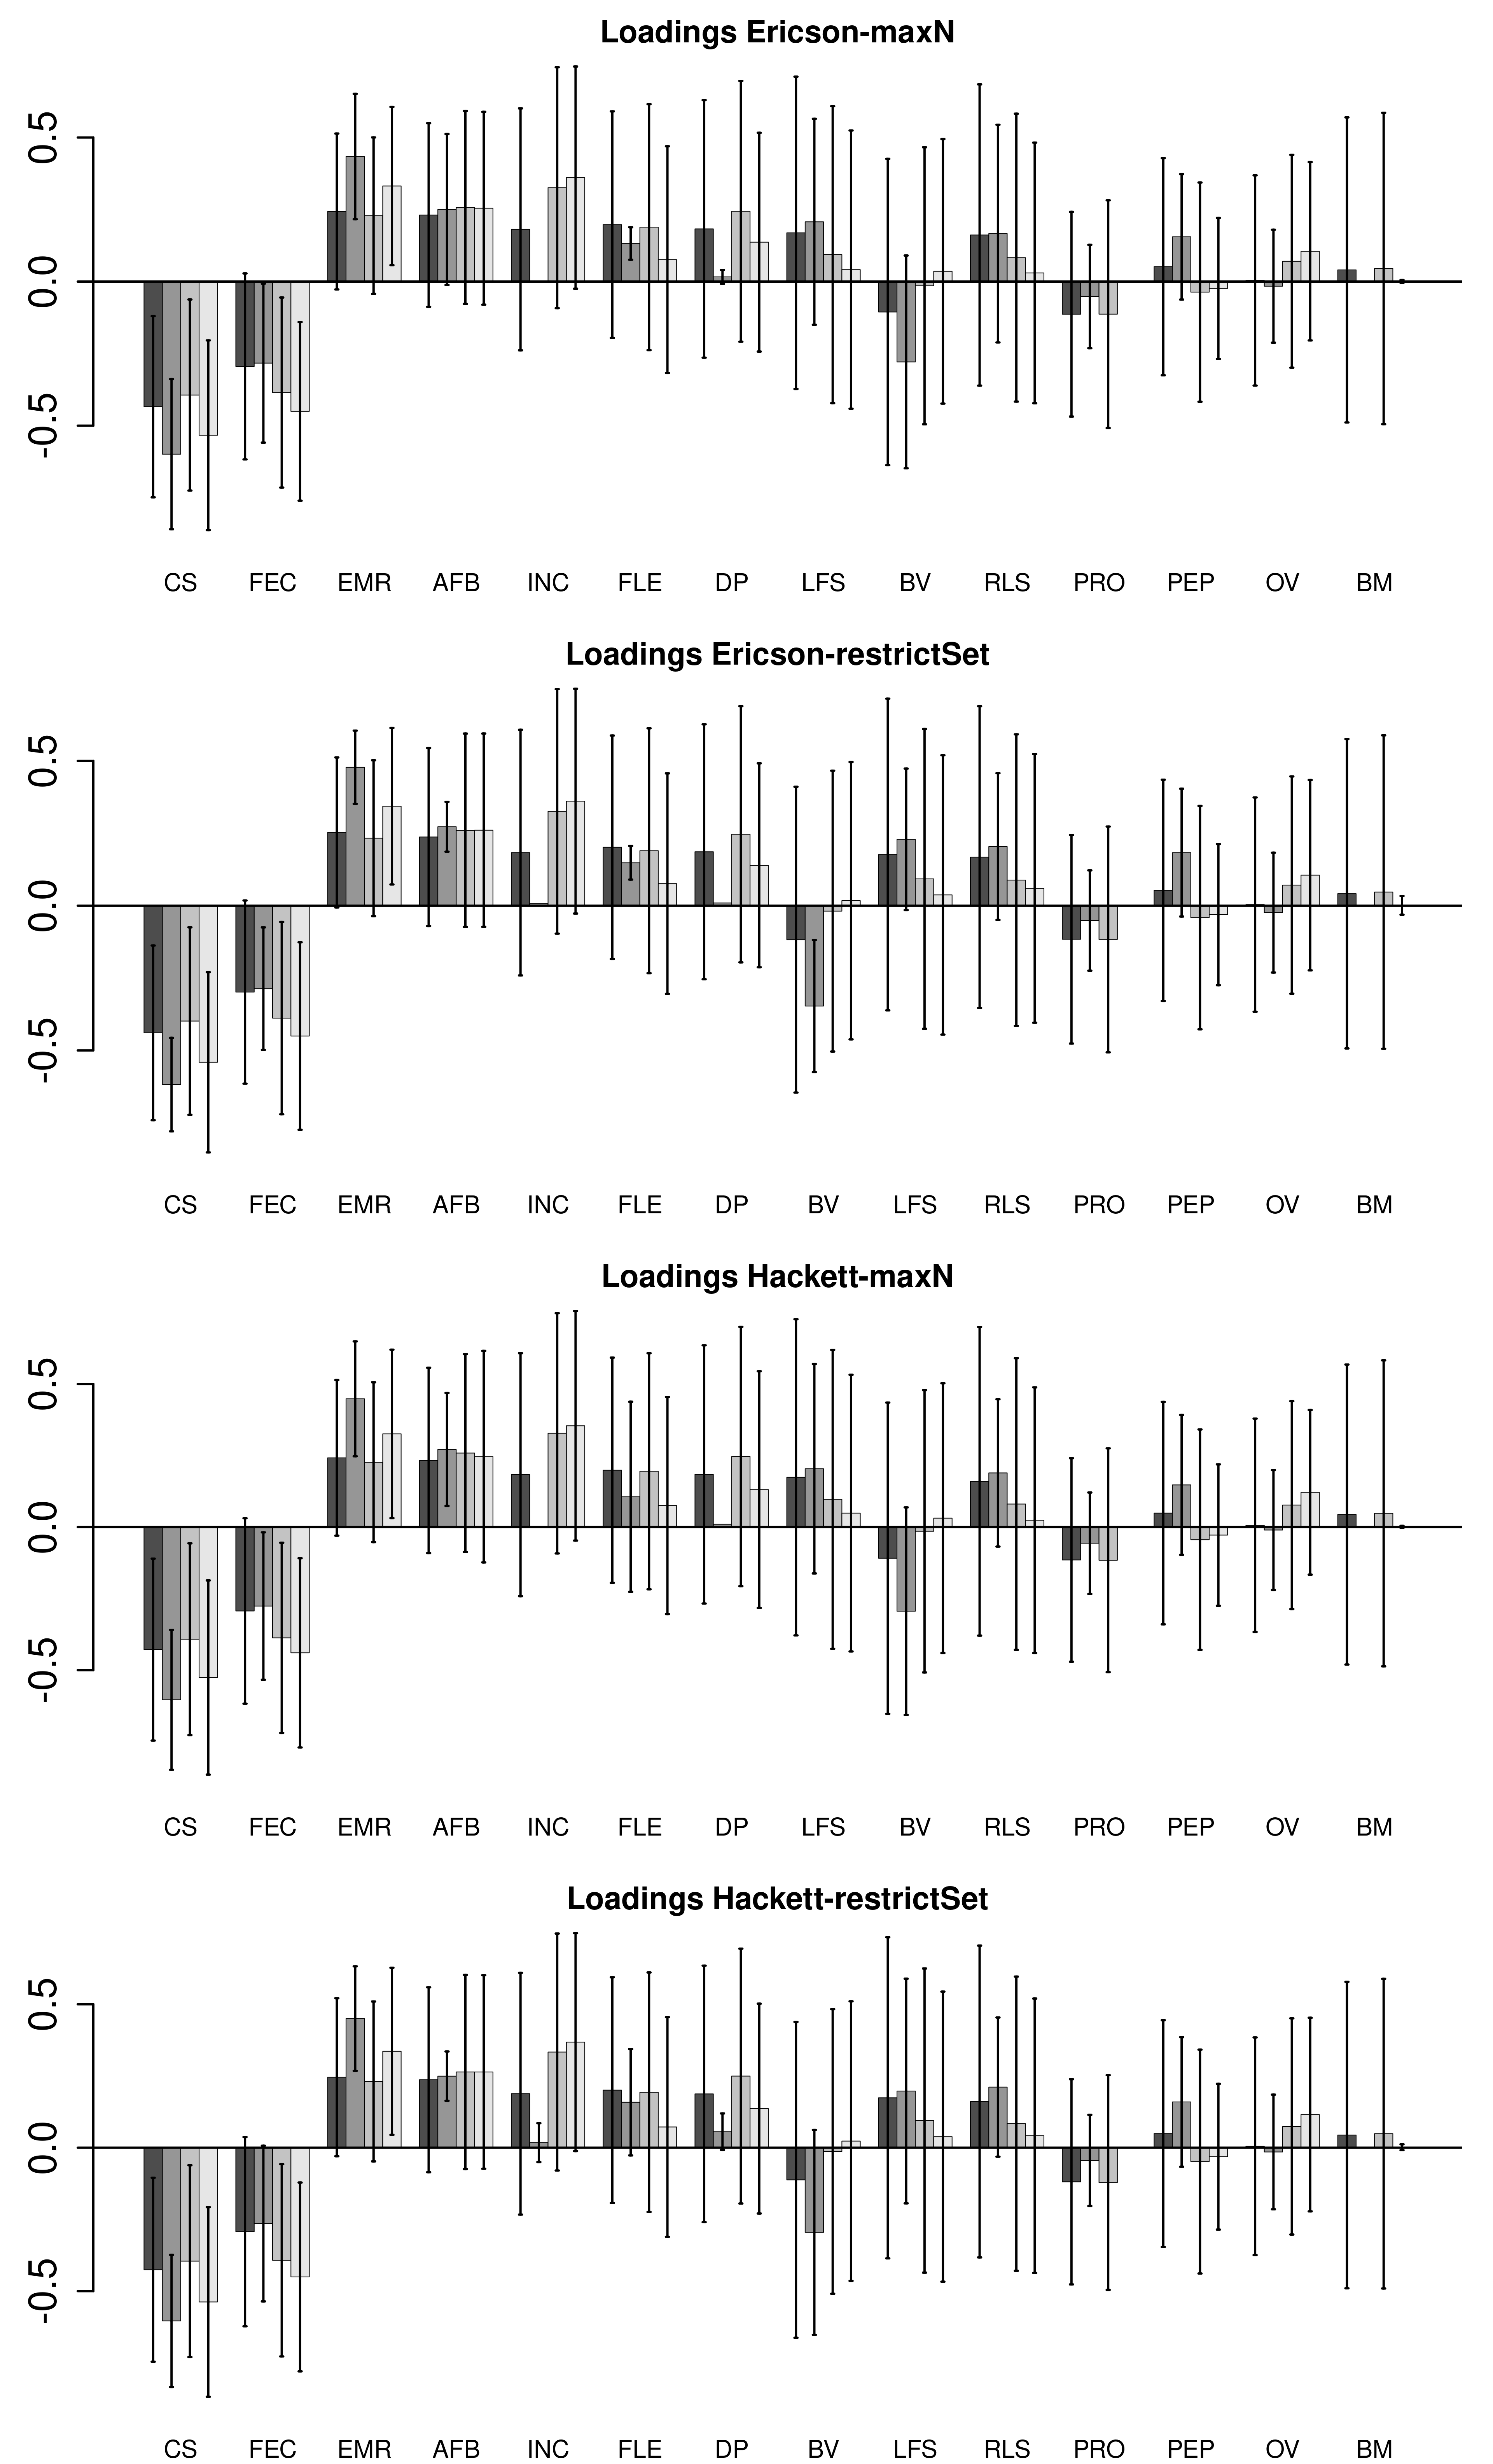
\includegraphics[width=.8\textwidth]{./Figures/Appendix2_1/FS loadings plots-ALL.png}
\caption[LHT loadings of the FS axes]{
Mean $\pm$ standard deviation AIC weighted loadings of the traits for the
fast-slow axes based on models predicting generation time or elasticity to
fecundity for all trait combination PCs o using only the PCs with AIC
\textless{2} (best AIC). From darker to lighter color: FSe, FSe best AIC, FSgt
and FSgt best AIC.}
\label{fig:figApp2.1}
\end{figure}

\begin{figure}[ht!]
\centering
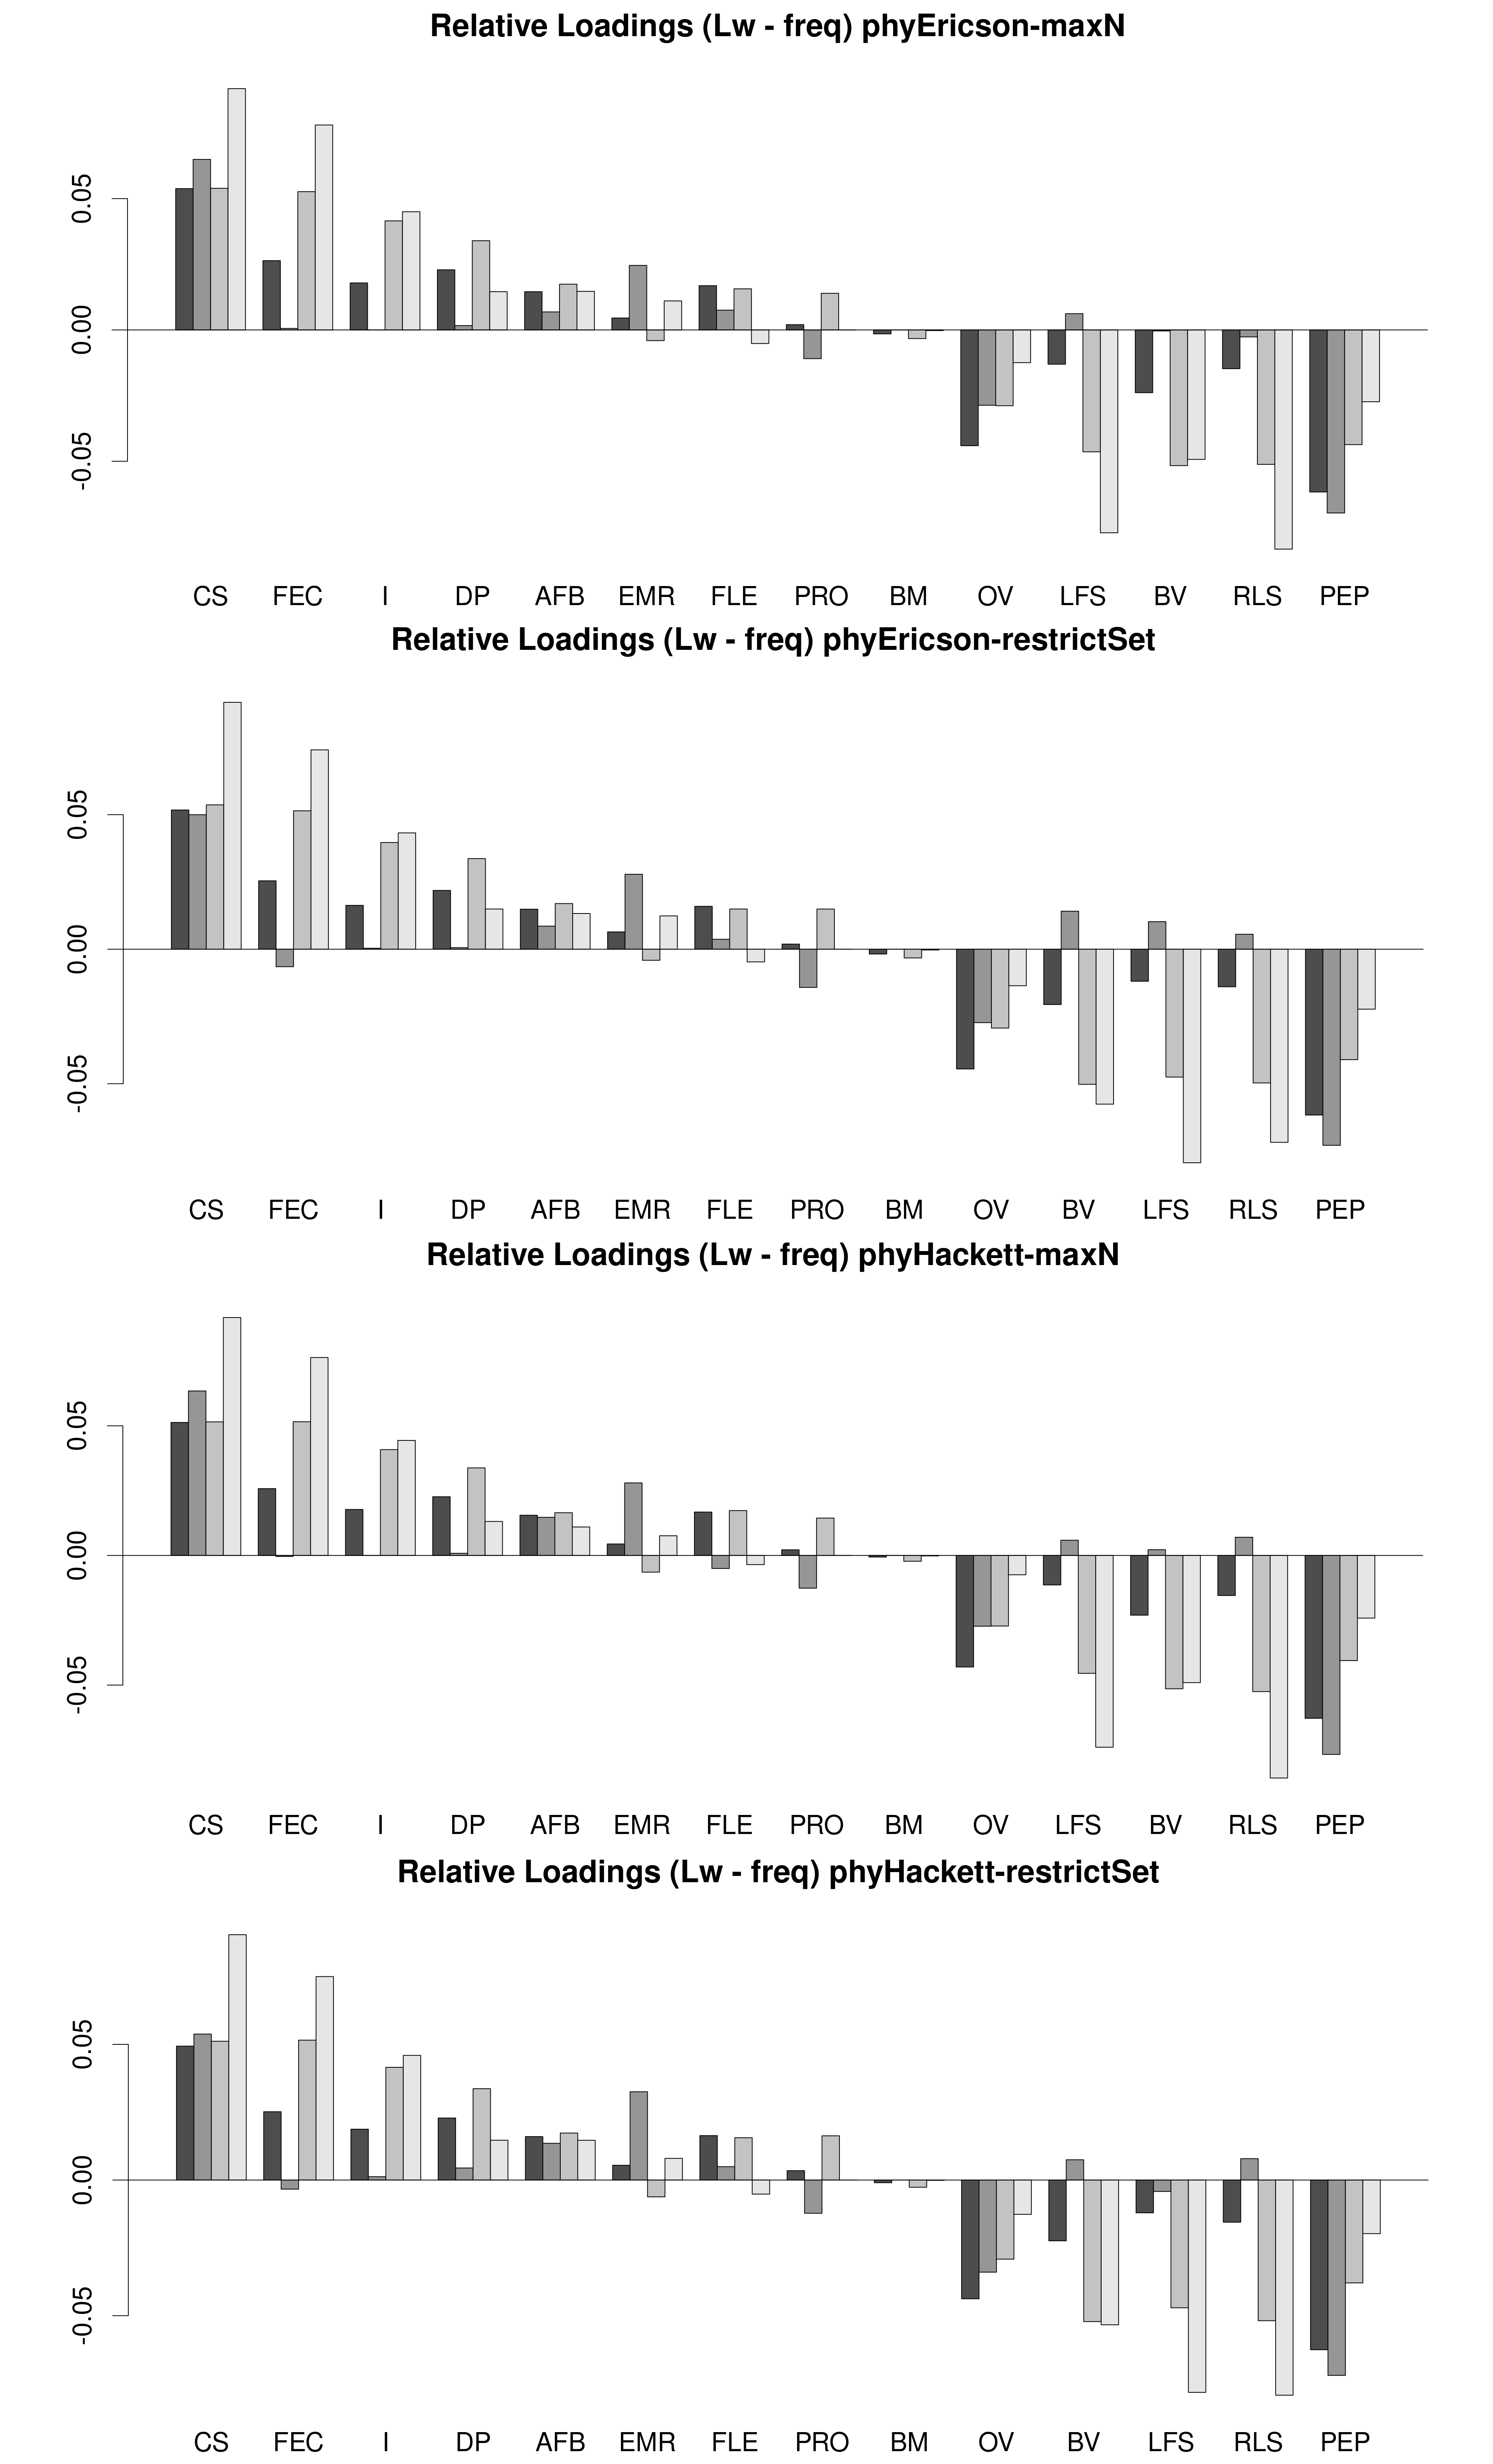
\includegraphics[width=.8\textwidth]{./Figures/Appendix2_1/FS relWeights plots-ALL.png}
\caption[LHT relative importance of the FS axes]{
Relative weight of the life history traits in the fast-slow continuum. Values
range from -1 to 1, where negative values means that the absolute value of the
trait loadings are lower than expected by the frequency of the trait and
positive values for traits with higher loadings than expected by the frequency
of the trait in the selected PPCAs (see main text for details). The loadings and
frequencies come from selected PCs that better predict elasticities to the
fecundity (FSe) or generation time (FSgt), weighted by the AIC based weight
of the models taking all or only the models with $\Delta AIC < 2$ (best AIC).
From darker to lighter color: FSe, FSe best AIC, FSgt and FSgt best AIC.}
\label{fig:figApp2.2}
\end{figure}

\begin{figure}[ht!]
\centering
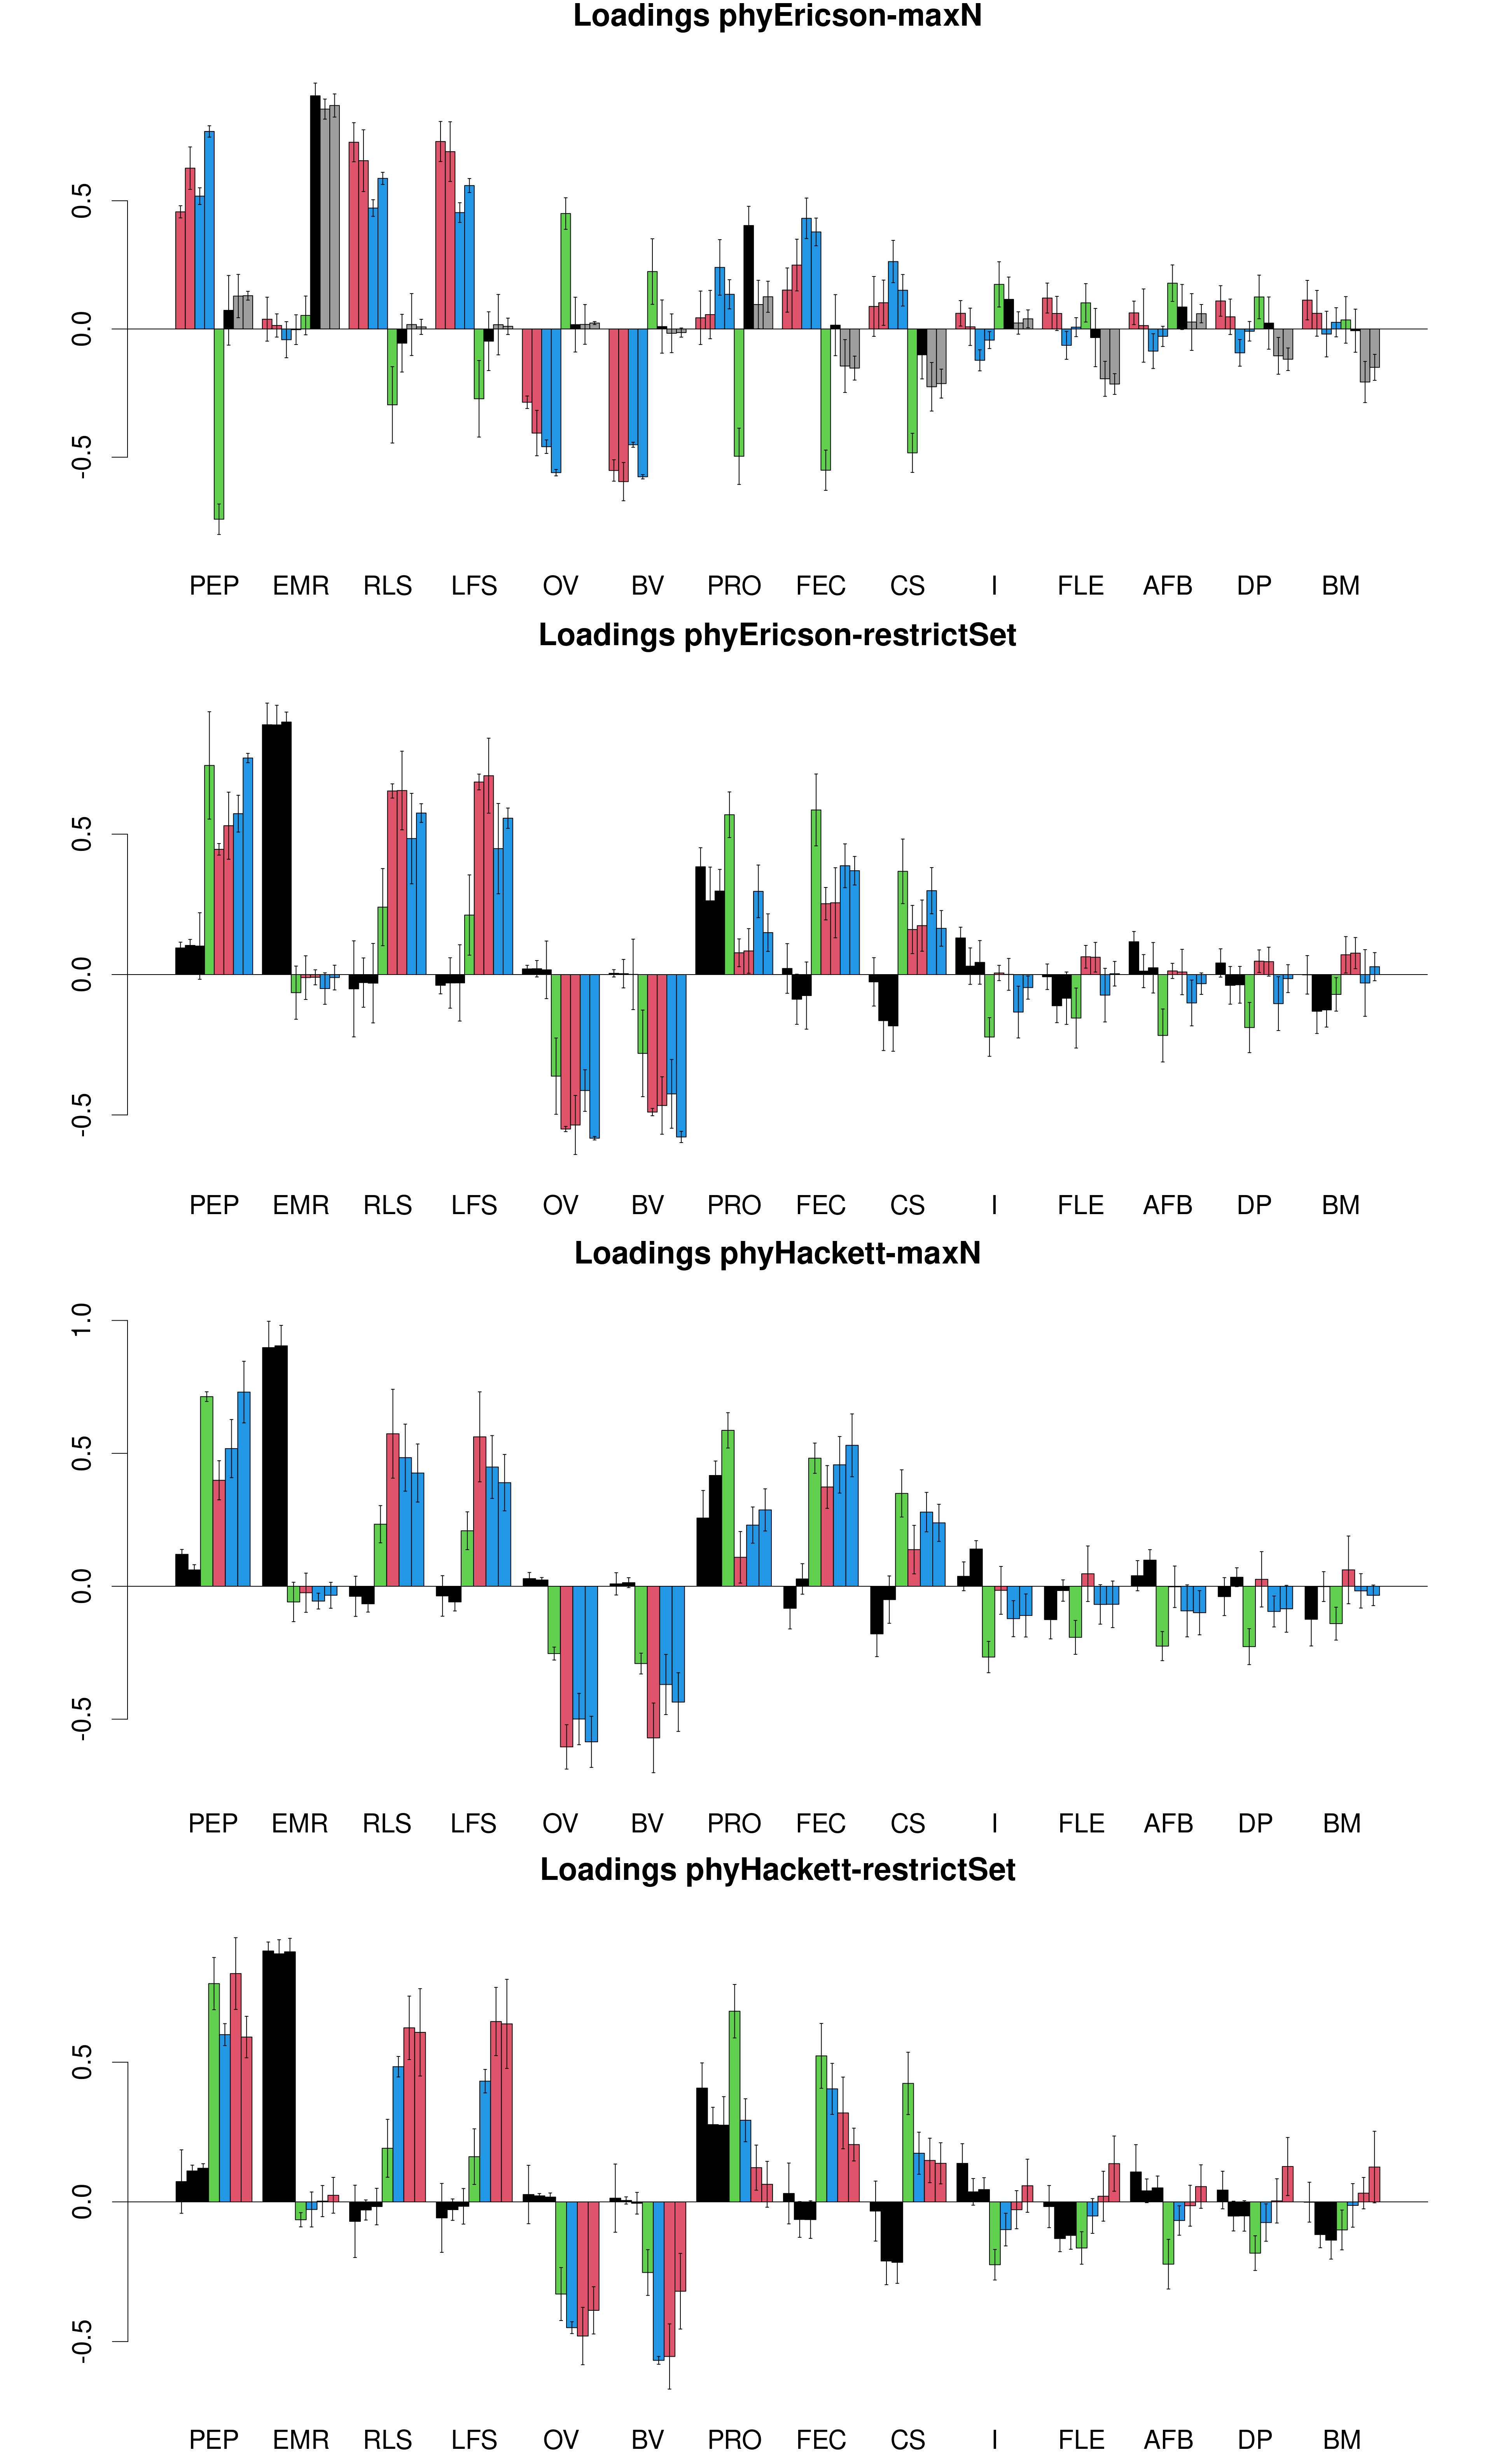
\includegraphics[width=.8\textwidth]{./Figures/Appendix2_1/2nd loadings plots-ALL.png}
\caption[LHT loadings of the secondary axes]{
Mean $\pm$ standard deviation of the loadings of the traits for clusters of
similar significant PCs (Eigenvalue \textgreater{1}) not selected for the
fast-slow axes. Groups follow the same order and colors than figure
\ref{fig:figApp2.5}.}
\label{fig:figApp2.3}
\end{figure}

\begin{figure}[ht!]
\centering
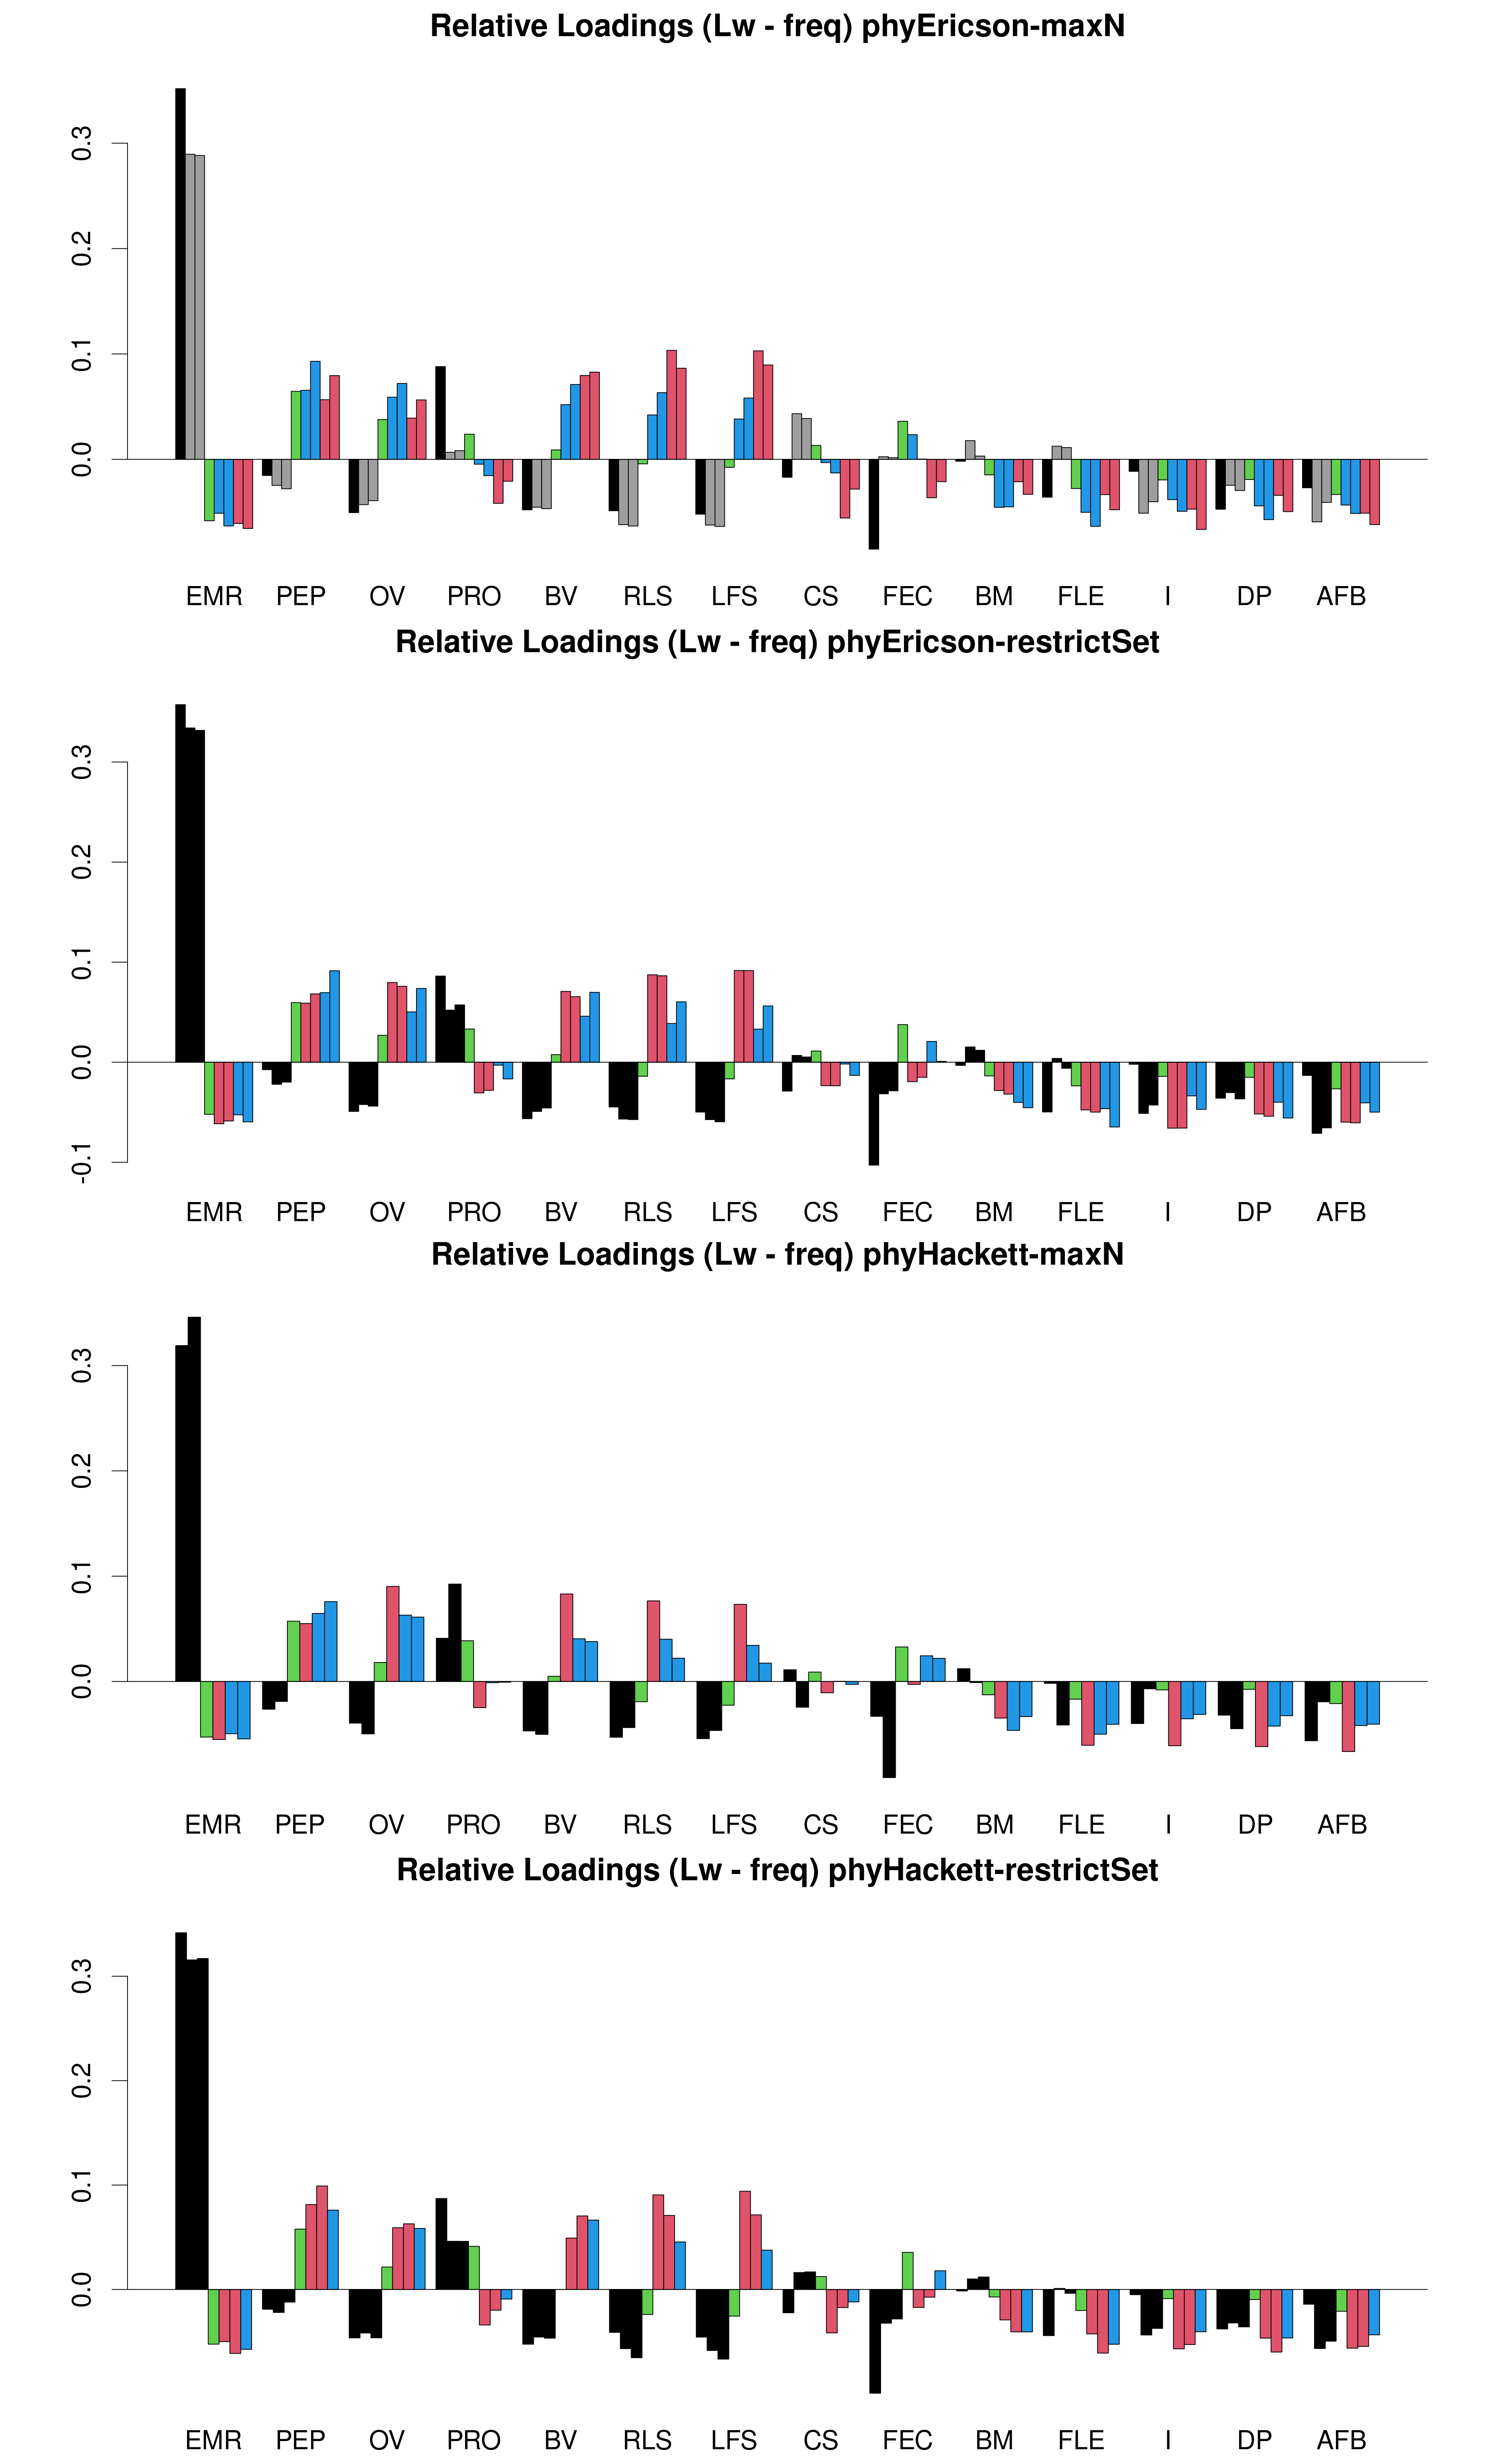
\includegraphics[width=.8\textwidth]{./Figures/Appendix2_1/2nd relWeights plots-ALL.png}
\caption[LHT relative importance of the secondary axes]{
Relative weights of the life history traits for each axes described in the
table \ref{tab:tabApp2.4}. Values range from -1 to 1, where negative values
means that the absolute value of the trait loadings are lower than expected by
the frequency of the trait and positive values for traits with higher loadings
than expected by the frequency of the trait in the selected PPCAs (see main
text for details). Groups follow the same order and colors as figure
\ref{fig:figApp2.5}.}
\label{fig:figApp2.4}
\end{figure}

\begin{figure}[ht!]
\centering
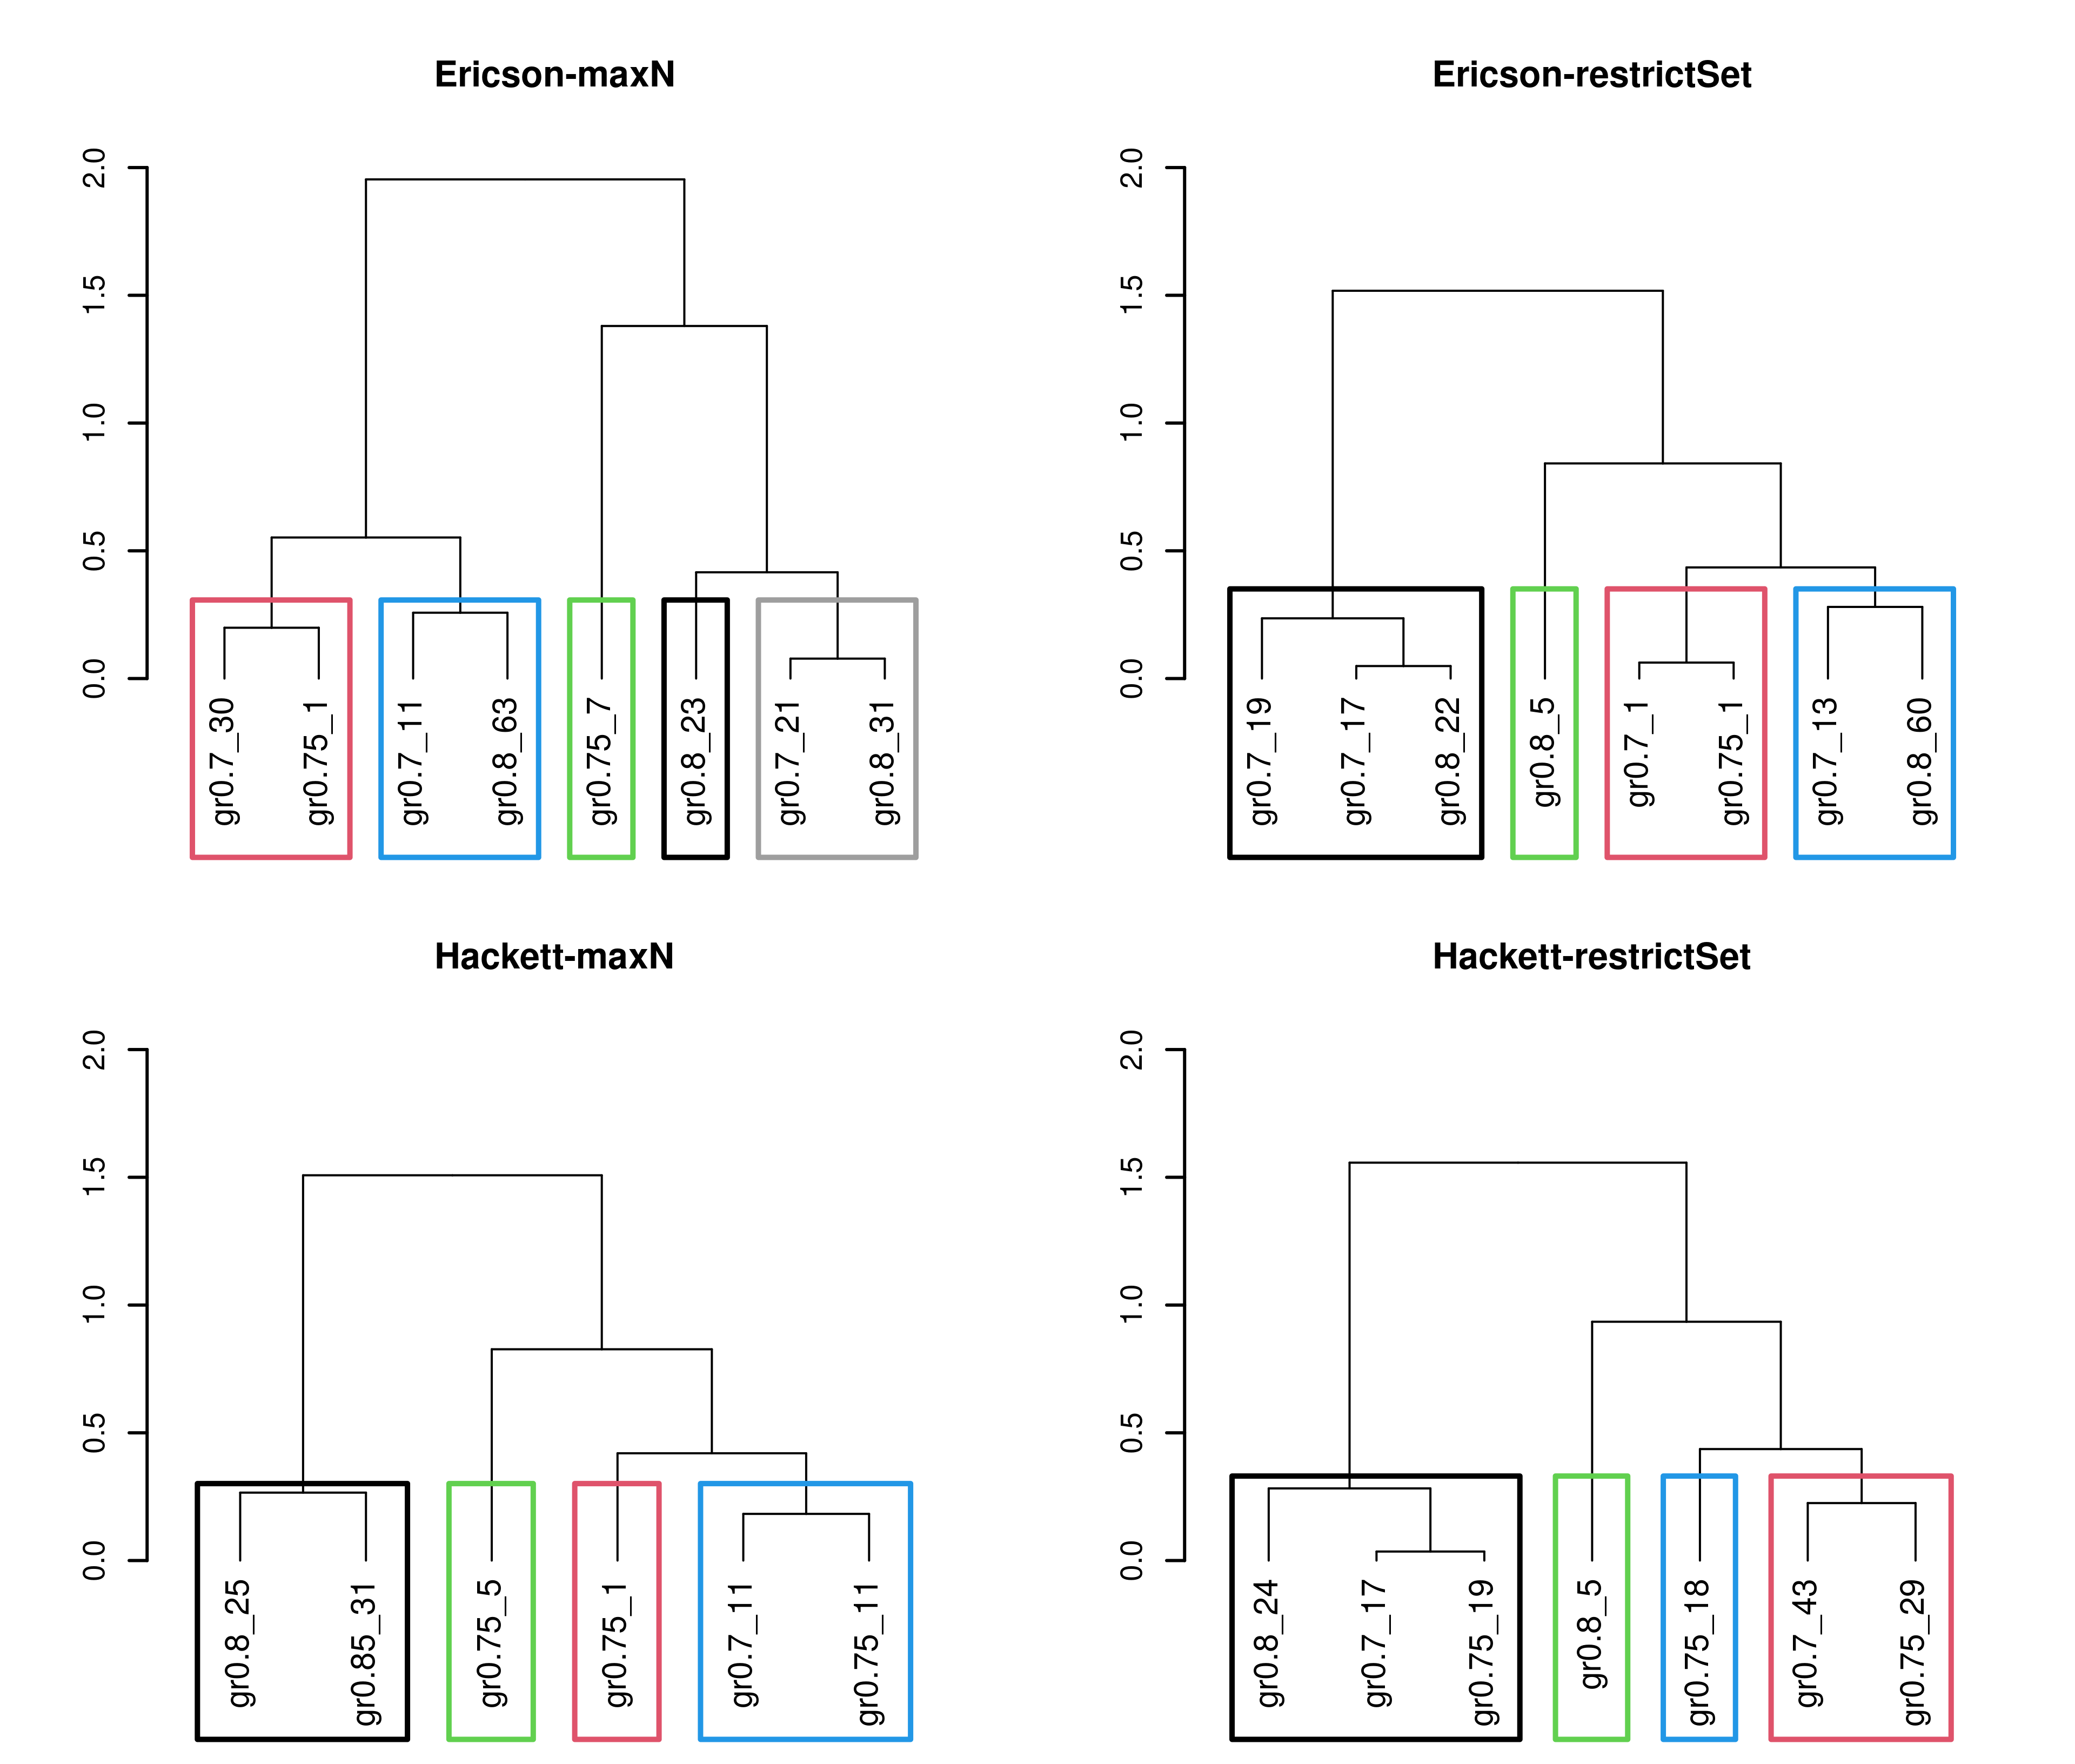
\includegraphics[width=.8\textwidth]{./Figures/Appendix2_1/2nd axes trees-1.png}
\caption[Cluster dendogram of the secondary axes]{
Dendogram of the distance among clusters of similar significant PCs (Eigenvalue
\textgreater{1}) not selected for the fast-slow axes. Each group contains PCs
with scores correlation greater than the correlation specified in the group name
(e.g. gr0.8 means correlation \textgreater{0.8}). Boxes include clusters with a
correlation among averaged loadings \textgreater{0.95} and can be conceptualized
as a offspring quality-quantity trade-off in black and grey, lifelong
productivity in green and iteroparity in blue and red.}
\label{fig:figApp2.5}
\end{figure}
